% Options for packages loaded elsewhere
\PassOptionsToPackage{unicode}{hyperref}
\PassOptionsToPackage{hyphens}{url}
%
\documentclass[
  12pt,
]{article}
\usepackage{amsmath,amssymb}
\usepackage{iftex}
\ifPDFTeX
  \usepackage[T1]{fontenc}
  \usepackage[utf8]{inputenc}
  \usepackage{textcomp} % provide euro and other symbols
\else % if luatex or xetex
  \usepackage{unicode-math} % this also loads fontspec
  \defaultfontfeatures{Scale=MatchLowercase}
  \defaultfontfeatures[\rmfamily]{Ligatures=TeX,Scale=1}
\fi
\usepackage{lmodern}
\ifPDFTeX\else
  % xetex/luatex font selection
\fi
% Use upquote if available, for straight quotes in verbatim environments
\IfFileExists{upquote.sty}{\usepackage{upquote}}{}
\IfFileExists{microtype.sty}{% use microtype if available
  \usepackage[]{microtype}
  \UseMicrotypeSet[protrusion]{basicmath} % disable protrusion for tt fonts
}{}
\makeatletter
\@ifundefined{KOMAClassName}{% if non-KOMA class
  \IfFileExists{parskip.sty}{%
    \usepackage{parskip}
  }{% else
    \setlength{\parindent}{0pt}
    \setlength{\parskip}{6pt plus 2pt minus 1pt}}
}{% if KOMA class
  \KOMAoptions{parskip=half}}
\makeatother
\usepackage{xcolor}
\usepackage[a4paper]{geometry}
\usepackage{color}
\usepackage{fancyvrb}
\newcommand{\VerbBar}{|}
\newcommand{\VERB}{\Verb[commandchars=\\\{\}]}
\DefineVerbatimEnvironment{Highlighting}{Verbatim}{commandchars=\\\{\}}
% Add ',fontsize=\small' for more characters per line
\usepackage{framed}
\definecolor{shadecolor}{RGB}{248,248,248}
\newenvironment{Shaded}{\begin{snugshade}}{\end{snugshade}}
\newcommand{\AlertTok}[1]{\textcolor[rgb]{0.94,0.16,0.16}{#1}}
\newcommand{\AnnotationTok}[1]{\textcolor[rgb]{0.56,0.35,0.01}{\textbf{\textit{#1}}}}
\newcommand{\AttributeTok}[1]{\textcolor[rgb]{0.13,0.29,0.53}{#1}}
\newcommand{\BaseNTok}[1]{\textcolor[rgb]{0.00,0.00,0.81}{#1}}
\newcommand{\BuiltInTok}[1]{#1}
\newcommand{\CharTok}[1]{\textcolor[rgb]{0.31,0.60,0.02}{#1}}
\newcommand{\CommentTok}[1]{\textcolor[rgb]{0.56,0.35,0.01}{\textit{#1}}}
\newcommand{\CommentVarTok}[1]{\textcolor[rgb]{0.56,0.35,0.01}{\textbf{\textit{#1}}}}
\newcommand{\ConstantTok}[1]{\textcolor[rgb]{0.56,0.35,0.01}{#1}}
\newcommand{\ControlFlowTok}[1]{\textcolor[rgb]{0.13,0.29,0.53}{\textbf{#1}}}
\newcommand{\DataTypeTok}[1]{\textcolor[rgb]{0.13,0.29,0.53}{#1}}
\newcommand{\DecValTok}[1]{\textcolor[rgb]{0.00,0.00,0.81}{#1}}
\newcommand{\DocumentationTok}[1]{\textcolor[rgb]{0.56,0.35,0.01}{\textbf{\textit{#1}}}}
\newcommand{\ErrorTok}[1]{\textcolor[rgb]{0.64,0.00,0.00}{\textbf{#1}}}
\newcommand{\ExtensionTok}[1]{#1}
\newcommand{\FloatTok}[1]{\textcolor[rgb]{0.00,0.00,0.81}{#1}}
\newcommand{\FunctionTok}[1]{\textcolor[rgb]{0.13,0.29,0.53}{\textbf{#1}}}
\newcommand{\ImportTok}[1]{#1}
\newcommand{\InformationTok}[1]{\textcolor[rgb]{0.56,0.35,0.01}{\textbf{\textit{#1}}}}
\newcommand{\KeywordTok}[1]{\textcolor[rgb]{0.13,0.29,0.53}{\textbf{#1}}}
\newcommand{\NormalTok}[1]{#1}
\newcommand{\OperatorTok}[1]{\textcolor[rgb]{0.81,0.36,0.00}{\textbf{#1}}}
\newcommand{\OtherTok}[1]{\textcolor[rgb]{0.56,0.35,0.01}{#1}}
\newcommand{\PreprocessorTok}[1]{\textcolor[rgb]{0.56,0.35,0.01}{\textit{#1}}}
\newcommand{\RegionMarkerTok}[1]{#1}
\newcommand{\SpecialCharTok}[1]{\textcolor[rgb]{0.81,0.36,0.00}{\textbf{#1}}}
\newcommand{\SpecialStringTok}[1]{\textcolor[rgb]{0.31,0.60,0.02}{#1}}
\newcommand{\StringTok}[1]{\textcolor[rgb]{0.31,0.60,0.02}{#1}}
\newcommand{\VariableTok}[1]{\textcolor[rgb]{0.00,0.00,0.00}{#1}}
\newcommand{\VerbatimStringTok}[1]{\textcolor[rgb]{0.31,0.60,0.02}{#1}}
\newcommand{\WarningTok}[1]{\textcolor[rgb]{0.56,0.35,0.01}{\textbf{\textit{#1}}}}
\usepackage{longtable,booktabs,array}
\usepackage{calc} % for calculating minipage widths
% Correct order of tables after \paragraph or \subparagraph
\usepackage{etoolbox}
\makeatletter
\patchcmd\longtable{\par}{\if@noskipsec\mbox{}\fi\par}{}{}
\makeatother
% Allow footnotes in longtable head/foot
\IfFileExists{footnotehyper.sty}{\usepackage{footnotehyper}}{\usepackage{footnote}}
\makesavenoteenv{longtable}
\usepackage{graphicx}
\makeatletter
\def\maxwidth{\ifdim\Gin@nat@width>\linewidth\linewidth\else\Gin@nat@width\fi}
\def\maxheight{\ifdim\Gin@nat@height>\textheight\textheight\else\Gin@nat@height\fi}
\makeatother
% Scale images if necessary, so that they will not overflow the page
% margins by default, and it is still possible to overwrite the defaults
% using explicit options in \includegraphics[width, height, ...]{}
\setkeys{Gin}{width=\maxwidth,height=\maxheight,keepaspectratio}
% Set default figure placement to htbp
\makeatletter
\def\fps@figure{htbp}
\makeatother
\setlength{\emergencystretch}{3em} % prevent overfull lines
\providecommand{\tightlist}{%
  \setlength{\itemsep}{0pt}\setlength{\parskip}{0pt}}
\setcounter{secnumdepth}{5}
\usepackage{fancyhdr}
\pagestyle{fancy}
\fancyhead{}
\fancyhead[R]{\small 2025-03-16}
\fancyhead[L]{\small Regression Linéaire}
\renewcommand{\headrulewidth}{0.4pt}
\usepackage[labelfont=bf, labelsep=colon, position=top]{caption} % Place la légende au-dessus de la figure
\ifLuaTeX
  \usepackage{selnolig}  % disable illegal ligatures
\fi
\usepackage{bookmark}
\IfFileExists{xurl.sty}{\usepackage{xurl}}{} % add URL line breaks if available
\urlstyle{same}
\hypersetup{
  pdfauthor={Dimitri DELPECH,; Timothé FADENIPO,; Matthis ARVOIS,; Ismael MADOU GAGI GREMA,; Cheikh LO},
  hidelinks,
  pdfcreator={LaTeX via pandoc}}

\title{\fbox{\huge Regression Linéaire}}
\author{Dimitri DELPECH, \and Timothé FADENIPO, \and Matthis
ARVOIS, \and Ismael MADOU GAGI GREMA, \and Cheikh LO}
\date{2025-03-16}

\begin{document}
\maketitle

{
\setcounter{tocdepth}{2}
\tableofcontents
}
\listoffigures

\listoftables

\newpage

\section{Introduction}\label{introduction}

(en cours)

\section{Revue empirique}\label{revue-empirique}

La résistance du béton est une propriété reconnue depuis longtemps. Si
le béton est un élément important du développement de nos sociétés,
c'est qu'il possède une résistance mécanique, en particulier à la
compression, qui a permis aux architectes et concepteurs de concevoir
des structures de plus en plus importantes et durables dans le temps. La
propriété de la résistance du béton reste la propriété la plus
importante du matériau pour du point de vue de l'ingénieur. Depuis
longtemps, la relation entre la composition du béton et la résistance au
béton fait écho dans le monde du génie civil et intéresse de nombreux
chercheurs de ce domaine. Cependant aucune théorie fondamentale et
universellement adoptée n'existe, en la matière, au-delà de la notion
commune de rapport eau/ciment. Cette première partie a pour but de
mettre en lumière les effets des variables explicatives sur la variable
cible en l'occurrence sur la résistance à la compression du béton en se
basant sur les travaux effectués dans ce sens.

Bien que dans toute approche fondamentale de la résistance à la
compression, la nature du granulat représente un rôle secondaire
néanmoins ceci reste important pour notre étude. Dans les années 1960,
Walker et Bloem ont publié dans leur article (Effect of Aggregate size
on properties of concrete, journal of AIC,septembre) un résultat assez
percutant. Il s'agit de la démonstration de l'effet négatif du volume de
la dimension maximale sur la résistance. Trois effets du granulat sur la
résistance du béton ont été énumérés à savoir un effet d'adhérence ;
l'effet de confinement et l'effet plafond (le Bulletin des Laboratoires
des Ponts et Chaussées, numéro 219, en janvier-février 1999, pages 41 à
52.).

A part son rôle important dans le phénomène de l'hydratation, l'eau est
l'un des facteurs les plus importants au niveau de l'ouvrabilité du
béton. L'augmentation du dosage en eau augmente la fluidité du béton et
entraîne la diminution de la concentration en solides. Cependant,
l'introduction excessive de l'eau provoque la chute de la résistance
mécanique et sa durabilité (effect on composition parameters on fresh
state properties of self-compacting concrete N.Bouhamou et al.). Le
bulletin publié par FEBELCEM (Fédération de l'Industrie Cimentière
Belge) avec l'auteur Ir C.Ployaert que la durabilité d'un béton dépend
d'une faible porosité. De plus, pour les surfaces de bétonnage non
coffrées sont les plus critiques du fait de leur exposition au soleil et
au vent. Le contrôle de leur protection efficace contre toute
évaporation intempestive de l'eau nécessaire à l'hydratation du ciment
revêt d'une grande importance. D'où la liaison importante entre la
résistance à la compression et l'eau.

Puis dans l'article publié par le département de génie civil à
l'université de Mostaganem en Algérie, le rôle de superplastifiant a été
mis en exergue. Le volume d'eau augmente avec l'augmentation du dosage
en superplastifiant. L'une des explications avancées est l'augmentation
de la viscosité de l'eau due au superplastifiant. De plus, il est noté
que l'augmentation du dosage en superplastifiant a engendré une
augmentation du taux de ségrégation statique dans le cas où le dosage
est élevé entraînant ainsi une réduction de l'homogénéité du béton et
par conséquent une réduction sa résistance à la compression. Par
ailleurs, un dosage modéré en superplastifiants apporte un bénéfice
supplémentaire, particulièrement aux premiers âges (48h, 72h), en raison
d'une meilleure compacité et d'une dispersion plus efficace des grains
de ciment.

Ensuite, Mehta et Monteiro (2014) soulignent que l'augmentation de la
teneur en ciment améliore significativement la résistance mécanique, en
particulier dans les premiers jours de durcissement. De même, Siddique
et al.~(2011) ont observé une corrélation positive entre la teneur en
ciment et la résistance à la compression, confirmant que cette relation
est particulièrement marquée dans les premières phases de durcissement.
Toutefois, au-delà d'un certain seuil, une concentration excessive de
ciment peut entraîner des effets négatifs, notamment une élévation de la
chaleur d'hydratation et une augmentation du retrait, favorisant ainsi
l'apparition de fissures (Neville, 2011). Il a également spécifié qu'il
existe une diminution dans l'efficacité du ciment en appliquant de très
haut dosage même en présence de superplastifiant dans ADDIS B.J ,
Alexandre M.G (1994) . Le dosage du ciment dans le béton est très
souvent relié à ses propriétés mécaniques et sa durabilité (effect on
composition parameters on fresh state properties of self-compacting
concrete N.Bouhamou et al.).

Par ailleurs, le laitier de haut fourneau est souvent utilisé pour
remplacer une partie du ciment afin d'améliorer certaines propriétés du
béton. Plusieurs études ont montré que son ajout réduit la résistance du
béton dans les premiers jours, car sa réaction est plus lente que celle
du ciment classique. Cependant, à plus long terme, il aide à renforcer
le béton grâce à une réaction chimique qui produit des éléments solides
supplémentaires, améliorant ainsi sa résistance (Jin et al., 2003).

De plus, l'utilisation des cendres volantes pour remplacer une partie du
ciment a aussi un impact sur la résistance du béton. D'après Tan et
al.~(2016), leur ajout réduit la résistance dans les premiers jours, car
elles réagissent plus lentement que le ciment. Toutefois, avec le temps,
elles renforcent la structure du béton et améliorent sa durabilité grâce
à une réaction chimique progressive. Zhao et al.~(2019) précisent que
leur effet dépend de la quantité utilisée et de la finesse des
particules, ce qui influence directement la résistance finale du béton.

En outre, Les granulats fins, communément appelés ``Fine Aggregate'',
constituent la fraction sableuse dans la formulation du béton. On
considère généralement qu'il s'agit de particules de dimensions
inférieures à 5 mm. La quantité de granulats fins, principalement
constitués de sable, influence la résistance du béton. Selon Chatterji
(2013), une bonne proportion de granulats fins améliore la compacité du
mélange, réduit la porosité et augmente la résistance à la compression.
Cependant, un excès de sable peut affaiblir la structure en diminuant la
cohésion entre les particules de ciment et les granulats plus gros
(Neville, 2011). Concrètement, une teneur adéquate en sable améliore le
contact entre la pâte cimentaire et les grains, réduisant la porosité et
favorisant ainsi un meilleur transfert des contraintes. Il est donc
essentiel de trouver un équilibre pour garantir une répartition homogène
des matériaux et optimiser la résistance du béton. Quant à l'étude du
bulletin des laboratoires des ponts et chaussées (1999) intitulée
``Influence du granulat sur la résistance à la compression des bétons'',
elle révèle qu'entre 60 \% et 75 \% de volume total d'agrégats, une
variation de la proportion de granulats fins peut entraîner un écart de
l'ordre de 2 à 3 MPa en résistance à la compression. La raison tient à
la formation d'une couche de pâte cimentaire plus ou moins épaisse selon
la quantité de sables incorporée, conditionnant ainsi la compacité et la
performance mécanique du béton. Enfin, L'âge du béton (Age) se définit
comme la durée écoulée depuis le coulage et le compactage jusqu'à la
réalisation des essais mécaniques, habituellement exprimée en nombre de
jours (1, 2, 7, 28, etc.). Il revêt une grande importance, car plus le
béton mûrit, plus la réaction d'hydratation du ciment se poursuit,
consolidant la microstructure et augmentant de manière significative la
résistance en compression. Plusieurs études, dont celles de Neville
(2011), Mindess et Young (2019), montrent que la résistance du béton
augmente avec le temps en raison du processus d'hydratation du ciment.
La majeure partie du gain de résistance se produit au cours des 28
premiers jours, période pendant laquelle le ciment continue de réagir
avec l'eau pour former une structure solide. Cependant, le taux de
durcissement ralentit après cette période, bien que certaines
formulations, notamment celles contenant du laitier ou des cendres
volantes, puissent encore voir leur résistance s'améliorer au-delà de 90
jours. Selon les observations présentées dans un mémoire de recherche
intitulé ``Impact du superplastifiant sur les propriétés
physico-mécaniques du ciment'' à l'université de Blida 1(2022-2023), la
résistance à la compression connaît une croissance rapide entre 1 et 7
jours, passant de 20 \% de la résistance ultime à près de 70 \% autour
de la première semaine . Typiquement, un saut d'environ 10 MPa (environ
50 \%) est constaté entre 2 et 7 jours. Après ce cap, le rythme de
durcissement ralentit, mais on atteint souvent plus de 90 \% de la
résistance finale à 28 jours.

\section{Zoom tour à tour sur les composantes de notre base de
données.}\label{zoom-tour-uxe0-tour-sur-les-composantes-de-notre-base-de-donnuxe9es.}

\subsection{Cement (voir annexe fig 1)}\label{cement-voir-annexe-fig-1}

L'histogramme montre une distribution étalée avec plusieurs pics,
indiquant une variabilité dans les proportions de ciment utilisées. Les
valeurs les plus courantes se situent entre 100 et 400 kg/m³. Cette
répartition suggère que différentes formulations de béton nécessitent
des proportions de ciment variées, influençant potentiellement la
résistance finale du béton.

\subsection{Blast Furnace Slag (voir annexe fig
2)}\label{blast-furnace-slag-voir-annexe-fig-2}

La majorité des valeurs sont proches de zéro, suggérant que le blast
furnace slag est rarement utilisé en grande quantité. Cependant,
quelques observations montrent une présence significative de ce
composant, ce qui pourrait indiquer des formulations spécifiques
cherchant à améliorer certaines propriétés du béton, comme la durabilité
ou la résistance aux sulfates.

\subsection{Fly Ash (voir annexe fig
3)}\label{fly-ash-voir-annexe-fig-3}

La distribution est fortement biaisée vers zéro, montrant que le fly ash
est peu utilisé dans la majorité des échantillons. Seules quelques
observations présentent des valeurs plus élevées, ce qui indique que cet
additif est employé dans des mélanges spécifiques, probablement pour
optimiser la maniabilité ou réduire les coûts en substituant une partie
du cement.

\subsection{Water (voir annexe fig 4)}\label{water-voir-annexe-fig-4}

La répartition est relativement normale avec un pic autour de 200 kg/m³,
ce qui indique une quantité d'eau standardisée dans la plupart des
mélanges. Une consommation d'eau bien contrôlée est essentielle pour
assurer une bonne hydratation du ciment et éviter une porosité excessive
pouvant affaiblir le matériau.

\subsection{Superplasticizer (voir annexe fig
5)}\label{superplasticizer-voir-annexe-fig-5}

La plupart des valeurs sont proches de zéro, ce qui signifie que le
superplasticizer est peu utilisé dans de nombreux échantillons.
Cependant, certaines observations indiquent une utilisation plus
importante, ce qui peut être lié à des mélanges nécessitant une
meilleure fluidité tout en réduisant le rapport water/cement pour
maximiser la résistance finale.

\subsection{Coarse Aggregate (voir annexe fig
6)}\label{coarse-aggregate-voir-annexe-fig-6}

Le coarse aggregate suit une distribution centrée autour de 950-1000
kg/m³, ce qui montre une standardisation dans son utilisation. La
présence d'une quantité relativement constante de coarse aggregate est
essentielle pour garantir la stabilité et la résistance mécanique du
béton tout en minimisant la fissuration.

\subsection{Fine Aggregate (voir annexe fig
7)}\label{fine-aggregate-voir-annexe-fig-7}

La distribution est également centrée autour de 750-800 kg/m³, suggérant
une utilisation homogène du fine aggregate dans les différents mélanges
de béton. Une quantité bien maîtrisée de fine aggregate améliore la
compacité du béton et influe sur sa capacité de mise en œuvre et son
imperméabilité.

\subsection{Age (voir annexe fig 8 )}\label{age-voir-annexe-fig-8}

L'âge du béton est majoritairement faible, avec une concentration autour
de 28 jours. Quelques échantillons présentent des âges plus avancés,
jusqu'à un an. Cela reflète l'importance de la période de cure du béton,
puisque la résistance continue d'augmenter avec le temps grâce à
l'hydratation prolongée du cement.

\subsection{Concrete Compressive Strength (voir annexe fig
9)}\label{concrete-compressive-strength-voir-annexe-fig-9}

La concrete compressive strength suit une distribution proche d'une loi
normale, avec un pic autour de 40 MPa. Cela indique une variabilité
contrôlée de la résistance du béton. La concrete compressive strength
étant un paramètre clé, cette distribution montre que la plupart des
mélanges atteignent une performance attendue, bien qu'il existe des
échantillons avec des valeurs plus élevées ou plus faibles en fonction
des formulations utilisées.

\section{Analyse Bivariéé : Expliquons la résistance à la compression du
béton par nos
variables.}\label{analyse-bivariuxe9uxe9-expliquons-la-ruxe9sistance-uxe0-la-compression-du-buxe9ton-par-nos-variables.}

La matrice de corrélation en annexe va nous aider à voir les différents
liens de corrélation potentiels entre nos variables. Dans cette partie,
nous allons étudier et essayer de trouver les couples de variables
significativement dépendants. Il est important de trouver tous les
couples liés afin d'expliquer de manière optimale comment les variables
de notre base peuvent influer sur la résistance à la compression du
béton.

\subsection{Quantité de ciment et résistance du béton. (voir annexe fig
12)}\label{quantituxe9-de-ciment-et-ruxe9sistance-du-buxe9ton.-voir-annexe-fig-12}

Nous allons ici examiner si la quantité de ciment utilisée pour créer le
béton est significativement reliée à la résistance à la compression du
béton. En effet, nous pouvons d'abord observer la distribution de ces
deux variables à l'aide du graphique ci-dessous :

Cette visualisation des données nous donne une première impression du
lien potentiel entre ces deux variables. En étudiant plus précisément
ces deux variables avec un test de corrélation de Pearson, on se rend
compte qu'il y a un lien significatif : ces deux variables sont
positivement liées.

On peut alors dire que plus la quantité de ciment utilisée pour la
fabrication du béton est grande, plus la résistance à la compression de
ce béton sera importante. Le test final a donné un coefficient de
corrélation \(\rho\) de Pearson égal à \textbf{0,5} (annexe), ce qui
indique un lien relativement fort et non négligeable. Ainsi, une
fabrication de béton comprenant une grande quantité de ciment
favoriserait grandement sa résistance à la compression.

\subsection{Additif chimique et eau. (voir annexe fig
13)}\label{additif-chimique-et-eau.-voir-annexe-fig-13}

Dans le processus de fabrication du béton, il est parfois nécessaire
d'ajouter un additif chimique pour améliorer sa fluidité et sa
maniabilité. La réflexion porte ici sur la corrélation entre l'ajout de
cet additif chimique et la quantité d'eau utilisée pour la fabrication :
y aurait-il un quelconque lien entre ces deux variables ?

Pour ce faire, il semble juste d'examiner les différents ajouts
d'additif en fonction de la quantité d'eau utilisée pour chaque béton.
Le graphique ci-dessous illustre cette relation, et nous pouvons
aisément supposer qu'il existe une corrélation entre ces deux variables.
En effet, dans l'ensemble, on remarque une diminution de l'ajout
d'additif lorsque la quantité d'eau augmente.

Pour avoir une certitude, nous effectuons alors un test de corrélation
de Kendall, qui nous indique, premièrement, qu'il existe un lien
significatif entre ces deux variables et, deuxièmement, que le
coefficient de corrélation \(\tau\) étant de \textbf{-0.53} (annexe), la
négativité de la liaison est prouvée.

En clair, plus la quantité d'eau utilisée pour la fabrication du béton
est importante, moins d'additif chimique a été ajouté lors de cette
fabrication. Ce lien fort nous aidera dans la suite de notre étude.

\subsection{L'age, une variable importante. (voir annexe fig
14)}\label{lage-une-variable-importante.-voir-annexe-fig-14}

Il serait tout à fait naturel de penser que l'âge ait une quelconque
importance sur la résistance à la compression du béton. En effet,
l'imaginaire collectif nous amène d'abord à penser que ce béton, en
conséquence de l'âge, deviendrait de plus en plus fragile et, de ce
fait, moins résistant à la compression. Notre hypothèse serait alors de
dire que l'âge est négativement lié à la résistance à la compression du
béton, \(i.e.\), plus l'âge augmente, moins le béton est résistant.

Dans un premier temps, l'observation de la distribution du temps par
rapport à la compression nous aiderait à confirmer ou infirmer
l'hypothèse de cette partie. Voyons le graphique ci-dessous.

Cette première visualisation ne nous permet pas de déterminer s'il
existe réellement un lien entre ces deux variables. Une exagération
pourrait peut-être nous amener à supposer l'existence d'une relation
quadratique entre elles, mais cette hypothèse ne peut être vérifiée dans
cette partie.

En conséquence, il est nécessaire de réaliser un test de corrélation.

Le test effectué nous permet de constater que notre hypothèse est
infirmée, car il existe bien un lien significatif entre ces deux
variables, et la corrélation indique que ce lien est positif. Cette
corrélation est positive mais modérée, avec un coefficient de Kendall
\(\tau\) de 0,449 (voir annexe). Les valeurs croissent significativement
ensemble, bien que certaines exceptions subsistent.

\subsection{La resistance à la compression du béton peut-elle
s'expliquer grâce au laitier de haut fournaux ? (voir fig
15)}\label{la-resistance-uxe0-la-compression-du-buxe9ton-peut-elle-sexpliquer-gruxe2ce-au-laitier-de-haut-fournaux-voir-fig-15}

On examine ici la relation entre le laitier de haut fourneau et la
résistance à la compression du béton :

Ce graphique ne suggère aucun lien de corrélation entre la quantité de
laitier de haut fourneau et la résistance à la compression du béton, mis
à part une légère baisse de la résistance du béton lorsque la quantité
de laitier de haut fourneau augmente. Afin de détecter une potentielle
relation de dépendance, il pourrait être judicieux d'effectuer un test
de corrélation de Spearman.

En effet, ce test nous fournit une p-value inférieure à 0.05 et un
coefficient \(\rho\) de 0.16. Ces valeurs indiquent qu'il existe bien un
lien significatif positif entre ces deux variables, mais cette
corrélation reste faible compte tenu de la proximité de \(\rho\) avec
zéro.

\subsection{Les cendres volantes peuvent-elles expliquer la resistance
du béton ? (voir annexe fig
16)}\label{les-cendres-volantes-peuvent-elles-expliquer-la-resistance-du-buxe9ton-voir-annexe-fig-16}

Pour tenter de répondre à cette question, on peut d'abord examiner la
distribution de la quantité de cendres volantes en fonction de la
résistance à la compression du béton.

La représentation de la distribution de notre variable à expliquer par
rapport à la variable explicative suggère une légère corrélation
linéaire négative. On pourrait alors en déduire que plus la quantité de
cendres volantes augmente, moins le béton résiste à la compression.

Pour s'assurer de la justesse de cette analyse, nous réalisons un test
de corrélation de Spearman, qui met en évidence un lien significatif
entre ces deux variables. Comme indiqué dans notre interprétation, ce
lien est négatif, avec un coefficient \(\rho\) de -0.19, indiquant ainsi
une corrélation faible mais non négligeable.

\subsection{L'eau, un facteur de résistance ? (voir Annexe fig
17)}\label{leau-un-facteur-de-ruxe9sistance-voir-annexe-fig-17}

Dans l'imaginaire collectif, il est tout à fait logique de penser que si
l'on ajoute de l'eau lors de la création du béton, celui-ci sera moins
résistant que si l'on ne le fait pas. Cependant, il est indispensable
d'incorporer une certaine quantité d'eau. L'objectif est donc de trouver
un juste milieu dans cette quantité. Examinons d'abord la distribution
de la résistance des bétons par rapport à leur résistance à la
compression :

Comme dans la partie précédente, le graphique est relativement
désordonné, mais on peut tout de même y relever une légère dépendance
négative, comme mentionné dans l'introduction de l'étude de cette
dépendance. Pour être sûr de nos analyses, il serait nécessaire
d'effectuer un test de corrélation de Spearman.

Le résultat de ce test indique qu'il existe bien une corrélation avec un
coefficient de corrélation de -0.31, ce qui montre un lien négatif non
négligeable entre ces deux variables.

En conclusion, moins il y a d'eau dans la création du béton, plus
celui-ci sera résistant. Cependant, les points situés à l'extrémité
gauche du graphique suggèrent qu'un minimum d'eau est tout de même
nécessaire pour que le béton atteigne une résistance suffisante.

\subsection{Superplasticité et Résistance (voir annexe fig
18)}\label{superplasticituxe9-et-ruxe9sistance-voir-annexe-fig-18}

Le superplastifiant, utilisé dans les mélanges de béton, joue un rôle
essentiel en améliorant la fluidité du béton sans ajout d'eau
supplémentaire. Ce composant chimique permet d'augmenter la densité du
béton, contribuant ainsi à une meilleure résistance à la compression.

Visuellement, le graphique ne permet pas de tirer de conclusions claires
sur la relation entre la quantité de superplastifiant et la résistance à
la compression du béton. Bien que la tendance semble indiquer une
augmentation initiale de la résistance avec l'ajout de superplastifiant,
la distribution des points reste dispersée. De plus, la présence de
nombreux points proches du début de la courbe rend difficile
l'identification d'une tendance nette.

Le test de Kendall révèle une corrélation positive modérée (tau = 0.249)
entre la quantité de superplastifiant et la résistance à la compression
du béton. Cette corrélation est significative, comme en témoigne la
p-value extrêmement faible, bien inférieure à 0.05. Cela suggère que, de
manière générale, une augmentation de la quantité de superplastifiant
dans le mélange de béton pourrait être associée à une amélioration de sa
résistance à la compression.

\subsection{Granulats grossiers et résistance à la compression (voir
annexe fig 19
)}\label{granulats-grossiers-et-ruxe9sistance-uxe0-la-compression-voir-annexe-fig-19}

Les granulats grossiers, qui comprennent des particules de grande taille
comme des graviers ou des pierres concassées, contribuent à la
résistance à la compression du béton en réduisant les vides dans le
mélange, augmentant ainsi sa compacité.

Le graphique représente la relation entre les granulats grossiers et la
résistance à la compression du béton. La répartition des données semble
dispersée. On peut néanmoins observer un lien quadratique entre ces deux
variables, mais il est difficile d'en tirer une conclusion plus
approfondie.

Le test de corrélation de Kendall a donné un coefficient tau de -0.124.
Bien que la p-value soit très faible (3.318e-09), ce faible tau indique
une relation négative mais modérée. Cela signifie qu'il existe bien une
certaine corrélation entre ces deux variables.

\subsection{Une relation floue entre les granulats fins et résistance à
la compression. ( voir annexe fig 20
)}\label{une-relation-floue-entre-les-granulats-fins-et-ruxe9sistance-uxe0-la-compression.-voir-annexe-fig-20}

La présence de granulats fins améliore la compacité du mélange, ce qui
peut influencer ses propriétés, notamment la résistance à la
compression. Ils remplissent les espaces entre les granulats plus
grossiers.

Le graphique des granulats fins ne permet pas de tirer de conclusions
claires concernant la relation entre cette variable et la résistance à
la compression, aucune tendance évidente n'y apparaît.

Les résultats du test de corrélation de Kendall indiquent une relation
significative entre la quantité de granulats fins et la résistance du
béton. Le coefficient \(\tau\) étant négatif, cela signifie que lorsque
la proportion de granulats fins diminue, la résistance à la compression
tend à augmenter. Cette observation suggère qu'un excès de granulats
fins pourrait réduire la compacité du mélange.

\section{Ingénierie des Données}\label{inguxe9nierie-des-donnuxe9es}

La base de données contient \textbf{1030 observations et 9 variables
numériques} initialement. Dans cette partie, nous préparons les données
pour garantir leur qualité et leur pertinence. Cette étape comprend deux
étapes principales :

\begin{itemize}
\tightlist
\item
  \textbf{Détection et traitement des valeurs aberrantes} à l'aide de
  boxplots.\\
\item
  \textbf{Analyse des corrélations} pour éviter la redondance des
  variables.
\end{itemize}

\subsection{Détection des valeurs
aberrantes}\label{duxe9tection-des-valeurs-aberrantes}

Les valeurs aberrantes peuvent fausser l'analyse et influencer la
modélisation. Les \textbf{boxplots} (voir
\hyperref[duxe9tection-des-valeurs-aberrantes-boxplots]{Analyse
univariée}) permettent d'identifier des observations extrêmes.

Certaines variables comme \textbf{Cement, Fly Ash} et \textbf{Coarse
Aggregate} ont une distribution homogène et sont conservées sans
modification.

La variable \textbf{Water} présente quelques valeurs extrêmes. Plutôt
que de les exclure, nous analysons leur impact.

La variable \textbf{Superplasticizer} contient des valeurs très
éloignées du reste des observations. Pour éviter toute influence
excessive, ces valeurs extrêmes sont exclues en utilisant la règle des
1.5*IQR :

\begin{Shaded}
\begin{Highlighting}[]
\CommentTok{\# Calcul des seuils avec la règle des 1.5*IQR pour Superplasticizer}
\NormalTok{Q1\_sp }\OtherTok{\textless{}{-}} \FunctionTok{quantile}\NormalTok{(bdd}\SpecialCharTok{$}\NormalTok{super\_plast, }\FloatTok{0.25}\NormalTok{)}
\NormalTok{Q3\_sp }\OtherTok{\textless{}{-}} \FunctionTok{quantile}\NormalTok{(bdd}\SpecialCharTok{$}\NormalTok{super\_plast, }\FloatTok{0.75}\NormalTok{)}
\NormalTok{IQR\_sp }\OtherTok{\textless{}{-}}\NormalTok{ Q3\_sp }\SpecialCharTok{{-}}\NormalTok{ Q1\_sp}

\NormalTok{seuil\_sup\_sp }\OtherTok{\textless{}{-}}\NormalTok{ Q3\_sp }\SpecialCharTok{+} \FloatTok{1.5} \SpecialCharTok{*}\NormalTok{ IQR\_sp}

\CommentTok{\# Filtrer les valeurs aberrantes pour Superplasticizer}
\NormalTok{bdd\_ing }\OtherTok{\textless{}{-}}\NormalTok{ bdd }\SpecialCharTok{\%\textgreater{}\%} \FunctionTok{filter}\NormalTok{(super\_plast }\SpecialCharTok{\textless{}=}\NormalTok{ seuil\_sup\_sp)}
\end{Highlighting}
\end{Shaded}

Concernant \textbf{Blast Furnace Slag}, quelques valeurs sont élevées
mais restent plausibles. Elles sont conservées sans modification.

La variable \textbf{Age} présente des valeurs extrêmes qu'il faut
filtrer. En utilisant la règle des 1.5*IQR, nous identifions les
observations anormalement élevées et les supprimons pour assurer une
meilleure cohérence des données :

\begin{Shaded}
\begin{Highlighting}[]
\CommentTok{\# Calcul des seuils avec la règle des 1.5*IQR pour Age}
\NormalTok{Q1\_age }\OtherTok{\textless{}{-}} \FunctionTok{quantile}\NormalTok{(bdd\_ing}\SpecialCharTok{$}\NormalTok{age, }\FloatTok{0.25}\NormalTok{)}
\NormalTok{Q3\_age }\OtherTok{\textless{}{-}} \FunctionTok{quantile}\NormalTok{(bdd\_ing}\SpecialCharTok{$}\NormalTok{age, }\FloatTok{0.75}\NormalTok{)}
\NormalTok{IQR\_age }\OtherTok{\textless{}{-}}\NormalTok{ Q3\_age }\SpecialCharTok{{-}}\NormalTok{ Q1\_age}

\NormalTok{seuil\_sup\_age }\OtherTok{\textless{}{-}}\NormalTok{ Q3\_age }\SpecialCharTok{+} \FloatTok{1.5} \SpecialCharTok{*}\NormalTok{ IQR\_age}

\CommentTok{\# Filtrer les valeurs aberrantes pour Age}
\NormalTok{bdd\_ing }\OtherTok{\textless{}{-}}\NormalTok{ bdd\_ing }\SpecialCharTok{\%\textgreater{}\%} \FunctionTok{filter}\NormalTok{(age }\SpecialCharTok{\textless{}=}\NormalTok{ seuil\_sup\_age)}
\end{Highlighting}
\end{Shaded}

\subsection{Analyse des corrélations}\label{analyse-des-corruxe9lations}

L'objectif est d'identifier les variables fortement corrélées entre
elles pour éviter la \textbf{multicolinéarité} dans le modèle.

La \textbf{matrice de corrélation} (voir
\hyperref[matrice-de-correlation]{Analyse bivariée}) permet d'observer
les liens entre les différentes variables.

La variable cible \textbf{y\_concrete\_compresive} présente des
corrélations notables avec certaines variables explicatives : -
\textbf{cement (0.50)} : Forte corrélation positive, suggérant une
relation directe entre la quantité de ciment et la résistance à la
compression.\\
- \textbf{cater (-0.29)} : Corrélation négative, ce qui est cohérent
avec l'hypothèse qu'un excès d'eau diminue la résistance du béton.\\
- \textbf{super\_plast (0.37)} : Corrélation indiquant que cet additif
pourrait améliorer la résistance du béton.\\
- \textbf{age (0.33)} : Relation positive, confirmant que la résistance
augmente avec le temps.

Certaines variables explicatives montrent également des
\textbf{corrélations importantes entre elles}, ce qui peut poser
problème : - \textbf{water et super\_plast (-0.65)} : Corrélation
négative forte, ce qui est logique car le superplastifiant permet de
réduire la quantité d'eau nécessaire.\\
- \textbf{blast\_furnace et fly\_ash (-0.32)} : Corrélation négative
modérée, indiquant que ces composants sont parfois utilisés en
substitution l'un de l'autre.

Nous devons \textbf{évaluer l'impact de ces relations dans le modèle}.
Si deux variables sont trop fortement corrélées, l'une d'elles pourrait
être supprimée pour éviter des problèmes de multicolinéarité.

Ces observations pourront nous aider lors de la sélection des variables
dans la prochaine étape.

\subsection{Synthèse de l'Ingénierie des
Données}\label{synthuxe8se-de-linguxe9nierie-des-donnuxe9es}

Après le traitement des valeurs aberrantes et l'analyse des
corrélations, la base de données passe de \textbf{1030 à 961
observations}.

Les valeurs extrêmes des variables \textbf{Age} et
\textbf{Superplasticizer} ont été supprimées en appliquant la règle des
1.5*IQR, garantissant une meilleure cohérence des données.

L'analyse des corrélations a révélé des relations notables entre
plusieurs variables, notamment une forte corrélation entre \textbf{Water
et Superplasticizer (-0.65)} et un lien important entre \textbf{Cement
et la résistance à la compression (0.50)}.

\section{Analyse Multivariée}\label{analyse-multivariuxe9e}

Dans cette partie, nous allons étudier l'ensemble des variables en
utilisant une analyse en composantes principales (ACP). La variable à
expliquer (``y\_concrete\_compresive'') est également considérée comme
active, aux côtés des huit autres variables explicatives.

\subsection{Histogramme des valeurs
propres}\label{histogramme-des-valeurs-propres}

\begin{verbatim}
## Warning: package 'FactoMineR' was built under R version 4.4.2
\end{verbatim}

\begin{center}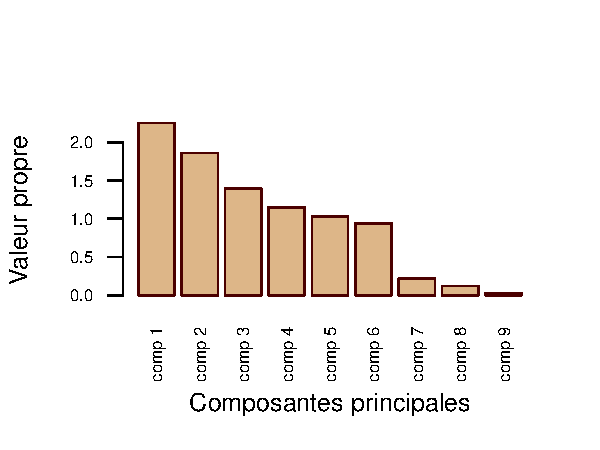
\includegraphics{rmd_final_files/figure-latex/unnamed-chunk-10-1} \end{center}

Le graphique illustre l'histogramme des valeurs propres issu de l'ACP,
permettant d'identifier le nombre d'axes principaux à retenir.

\begin{itemize}
\tightlist
\item
  Le premier axe capte une part importante de la variance totale.
\item
  Le deuxième axe conserve également une proportion significative
  d'information.
\item
  Le troisième axe ajoute un complément notable de variance.
\item
  À partir du quatrième axe, la contribution devient plus marginale.
\end{itemize}

En appliquant la \textbf{règle du coude}, il est pertinent de retenir
les \textbf{trois premiers axes} pour l'analyse.

\subsection{Analyse sur les 2 Premiers
Axes}\label{analyse-sur-les-2-premiers-axes}

\begin{center}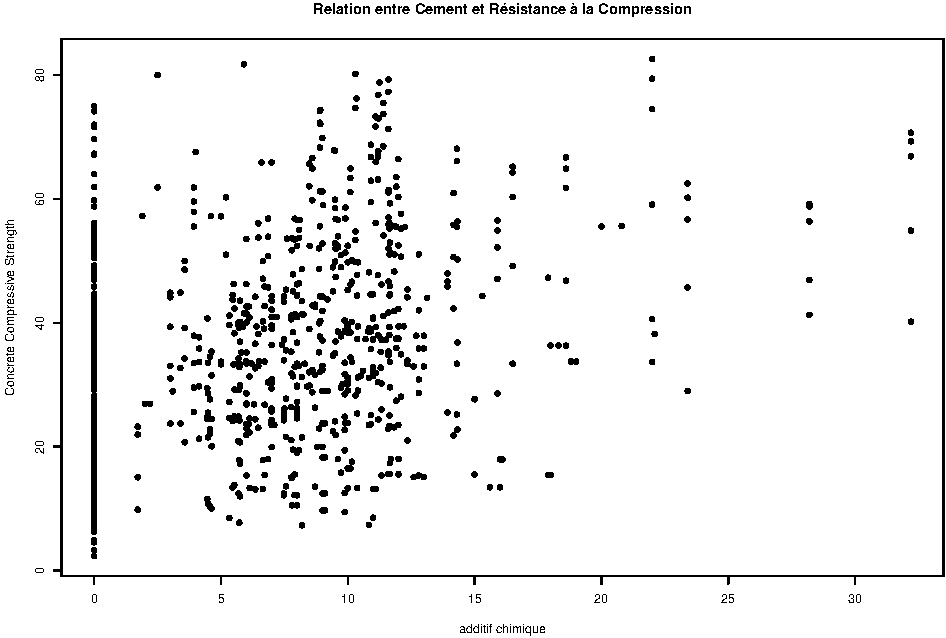
\includegraphics{rmd_final_files/figure-latex/unnamed-chunk-11-1} \end{center}

Le cercle de corrélation met en évidence les relations entre les
variables étudiées, projetées sur les deux premiers axes principaux de
l'ACP. Ces axes capturent ensemble \textbf{45,67 \%} de la variance
totale des données (\textbf{25,02 \% pour Dim 1 et 20,64 \% pour Dim
2}).

\subsubsection{Interprétation du Premier Axe (Dim 1 : 25,02
\%)}\label{interpruxe9tation-du-premier-axe-dim-1-2502}

Le premier axe distingue \textbf{les formulations riches en eau
(\texttt{water})} de celles utilisant \textbf{des superplastifiants
(\texttt{super\_plast})}.

\begin{itemize}
\tightlist
\item
  \texttt{water} (28,20 \% de contribution, cos² = 0.62) est la deuxième
  variable la plus influente sur Dim 1. Son orientation négative indique
  qu'une teneur élevée en eau tend à être associée à une baisse de la
  résistance à la compression.
\item
  \texttt{super\_plast} (30,77 \% de contribution, cos² = 0.69) est
  projetée dans la direction opposée à \texttt{water}, traduisant son
  rôle de réduction du besoin en eau, favorisant ainsi la résistance.
  c'est la variable la plus influente sur cet axe.
\item
  \texttt{fly\_ash} (7,3 \% de contribution, cos² = 0.16) et
  \texttt{fine\_aggr} (4,86\% de contribution, cos² = 0.11) ne sont pas
  bien projetées sur cet axe.
\item
  \texttt{age} (5,57 \% de contribution, cos² = 0.13) est aussi bien
  représenté sur Dim 1, confirmant que la résistance du béton augmente
  avec le temps de durcissement.
\item
  \texttt{y\_concrete\_compresive} (19,17 \% de contribution, cos² =
  0.43) est bien projetée sur Dim 1 ainsi que son cos² indique qu'elle
  est très bien representée sur cet axe.
\end{itemize}

\subsubsection{Interprétation du Deuxième Axe (Dim 2 : 21,52
\%)}\label{interpruxe9tation-du-deuxiuxe8me-axe-dim-2-2152}

Le deuxième axe distingue \textbf{les formulations riches en ciment
(\texttt{cement}) et associées à une plus grande résistance
(\texttt{y\_concrete\_compresive})} des formulations utilisant
\textbf{une proportion plus élevée des cendres volantes (`fly\_ash') et
les granulats fins (\texttt{fine\_aggr})}.

\begin{itemize}
\tightlist
\item
  \texttt{y\_concrete\_compresive} (24.70 \% de contribution, cos² =
  0.45) est la variable la plus influente sur Dim 2. Cela signifie que
  la résistance à la compression est fortement expliquée par cette
  dimension.
\item
  \texttt{cement} (21.78 \% de contribution, cos² = 0.40) est bien
  représentée sur Dim 2, indiquant que la quantité de ciment influence
  fortement la résistance mécanique. -fly\_ash (20.39\% de contribution
  et cos² = 0.38) et fin\_aggr (13.01\% de contribution et cos² = 0,24)
  contribuent plus sur cet axe que sur le premier et elles sont très
  bien representées sur cet axe contrairement au premier axe, suggérant
  que ces composants influencent la résistence du béton de la meme façon
  puisque les fleches de ces deux variables sont confondues.
\item
  \texttt{coarse} (5.05 \% de contribution, cos² = 0.10) et
  blast\_furnace (10.61\% de contribution et un cos² = 0.10) ne sont pas
  bien projetées sur cet axe et contribue faiblement à al construction
  de cette dimension. Elles pourraient etre expliquées par le troisième
  axe.
\end{itemize}

\subsection{Interprétation du Troisième
Axe}\label{interpruxe9tation-du-troisiuxe8me-axe}

\subsubsection{Dim(1-3) : 40.5\% \% de la Variance Totale (Voir annexe :
fig 21)}\label{dim1-3-40.5-de-la-variance-totale-voir-annexe-fig-21}

Le troisième axe distingue \textbf{les formulations riches en laitier du
haut fourneau (\texttt{blast\_frunace}) et associées à une plus grande
résistance (\texttt{y\_concrete\_compresive})} des formulations
utilisant \textbf{une proportion plus élevée des granulats grossiers
(\texttt{Coarse}) et du ciment (\texttt{Cement})}. ces deux axes
representent 40.5\% de la varaince totale.

-\texttt{blast\_frunace} (38.12\% de contribution et cos² = 0.53)
constitue la variable la plus influente et impacte positivement la
resistance à la compression du beton. une hausse du laitier haut
fourneau renforce la resistance.

-\texttt{Coarse} (avec 32.5\% de contribution et cos² = 0.45) represente
la deuxieme variable la plus importante et contribue en grande partie à
la construction de cet axe. elle est projetée dans la direction opposée
à \texttt{blast\_frunace} et \texttt{y\_concrete\_compresive}, suggérant
que les formulations contenant une proportion élevée de granulats
grossiers sont associées à une résistance plus faible.

\begin{itemize}
\tightlist
\item
  Enfin, nous avons la variable \texttt{Cement} qui est egalement bien
  representée (cos² = 0.27) et contribue à la hauteur de 19.46\% à la
  construction de cet axe.
\end{itemize}

\subsubsection{Dim(2-3) : 36.14 \% de la Variance Totale (Voir annexe :
Partie
22)}\label{dim2-3-36.14-de-la-variance-totale-voir-annexe-partie-22}

Le troisième axe distingue \textbf{les formulations riches en laitier du
haut fourneau (\texttt{blast\_frunace}) et associées à une plus grande
résistance (\texttt{y\_concrete\_compresive})} des formulations
utilisant \textbf{une proportion plus élevée des granulats grossiers
(\texttt{Coarse}) et du ciment (\texttt{Cement})}. ces deux axes
representent 40.5\% de la varaince totale.

nous remarquons la meme conclusion que l'analyse des axes 1-3. Retenons
que la variable age (\texttt{age}) n'est pas bien representée sur les
trois premiers axes mais pon remmarque qu'elle est très bien representée
sur le quatrième axe avec 40.72\% de contribution et 0.46 comme qualité
de representation. compte tenu de la mauvaise representation de la
variable cible sur cet axe, nous pouvons conclure que l'age n'influence
pas de manière significative la resistance à la compression du beton.

Cette ACP met en évidence trois dimensions principales dans la
composition du béton :

\begin{enumerate}
\def\labelenumi{\arabic{enumi}.}
\tightlist
\item
  \textbf{Axe 1 (Dim 1)} : Opposition entre l'eau et les
  superplastifiants.
\item
  \textbf{Axe 2 (Dim 2)} : Opposition entre ciment et cendres volantes,
  granulats fins.
\item
  \textbf{Axe 3 (Dim 3)} : Opposition entre laitier du haut fourneau et
  granulats grossiers, ciment
\end{enumerate}

\subsection{Implications pour la Modélisation de la Résistance du
Béton}\label{implications-pour-la-moduxe9lisation-de-la-ruxe9sistance-du-buxe9ton}

\begin{itemize}
\tightlist
\item
  L'opposition entre \texttt{water} et \texttt{super\_plast} sur Dim 1
  indique qu'un \textbf{terme d'interaction} entre ces deux variables
  pourrait être testé dans le modèle linéaire.
\item
  \texttt{fine\_aggr} et \texttt{fly\_ash} étant bien projetées sur Dim
  2, leurs interactions avec \texttt{cement} pourraient être pertinentes
  pour examiner leurs effets combinés sur la compacité et la résistance.
\item
  \texttt{age} étant bien représentée sur Dim 4, une interaction avec
  \texttt{Cement} pourrait être étudiée pour voir comment l'évolution du
  béton avec le temps est influencée par le ciment.
\item
  \texttt{y\_concrete\_compresive} étant principalement projeté sur Dim
  2, un modèle linéaire devrait inclure \textbf{\texttt{cement},
  \texttt{blast\_furnace}, \texttt{fly\_ash}, \texttt{fine\_aggr}} comme
  facteurs explicatifs car d'après nos analyses, ce sont les variables
  succeptibles d'influer sur la resistance à la compression.
\item
  L'opposition entre \texttt{coarse} et \texttt{super\_blast} sur Dim 2
  suggère qu'un effet combiné de ces deux variables pourrait influencer
  la résistance mécanique.
\end{itemize}

\section{Modélisation Linéaire}\label{moduxe9lisation-linuxe9aire}

\begin{longtable}[]{@{}lrrrl@{}}
\caption{Tableau des résultats de la régression linéaire}\tabularnewline
\toprule\noalign{}
Coefficient & Estimate & Std\_Error & t\_value & Pr \\
\midrule\noalign{}
\endfirsthead
\toprule\noalign{}
Coefficient & Estimate & Std\_Error & t\_value & Pr \\
\midrule\noalign{}
\endhead
\bottomrule\noalign{}
\endlastfoot
(Intercept) & -23.163756 & 26.588421 & -0.871 & 0.383851 \\
cement & 0.119785 & 0.008489 & 14.110 & \textless{} 2e-16 \\
blast\_furnace & 0.103847 & 0.010136 & 10.245 & \textless{} 2e-16 \\
fly\_ash & 0.087943 & 0.012585 & 6.988 & 5.03e-12 \\
water & -0.150298 & 0.040179 & -3.741 & 0.000194 \\
super\_plast & 0.290687 & 0.093460 & 3.110 & 0.001921 \\
coarse & 0.018030 & 0.009394 & 1.919 & 0.055227 \\
fine\_aggr & 0.020154 & 0.010703 & 1.883 & 0.059968 \\
age & 0.114226 & 0.005427 & 21.046 & \textless{} 2e-16 \\
\end{longtable}

\textbf{Interprétation des p-values}

Les résultats de la régression montrent que :

\begin{itemize}
\tightlist
\item
  \textbf{Intercept} : La p-value est de \textbf{0.38}, ce qui est
  \textbf{supérieur à 0.05}. Nous retenons donc l'\textbf{hypothèse H0},
  selon laquelle cette valeur n'est \textbf{pas significative}.
\item
  \textbf{Variables significatives (p \textless{} 0.05)} :
  \texttt{cement}, \texttt{blast\_furnace}, \texttt{fly\_ash},
  \texttt{water}, \texttt{super\_plast} et \texttt{age}. Nous acceptons
  l'\textbf{hypothèse H1}, qui indique que ces variables ont un
  \textbf{effet significatif} sur la résistance du béton.
\item
  \textbf{Variables non significatives au seuil de 5 \%} :
  \texttt{coarse} et \texttt{fine\_aggr}. Toutefois, elles deviennent
  \textbf{significatives pour un seuil de 10 \%}.
\end{itemize}

Ces résultats suggèrent que certaines variables ont un impact plus
marqué sur la \textbf{résistance à la compression du béton}, tandis que
d'autres jouent un rôle moins déterminant.

Au regard de ces variables significatives, nous avons constaté des
effets diverses sur la variable réponse. Pour la variable
\textbf{Cement}(ciment), on remarque un effet positif sur la variable
réponse qui n'est rien d'autre que la résistance à la compression. La
valeur de cette relation est de l'ordre de 0.119785, cela signifie que
si le ciment augmente d'une unité alors la résistence à la compression
augmente moins proportionnellement que l'augmentation du ciment (0.12
unité). Ensuite, pour la variable blast\_furnace (laitier de haut
fourneau), la relation est positive. Cela signifie qu'une hausse de la
variable en question d'une unité entraine une augmentation de 0.12 unité
de la variable cible. Puis, on s'interesse à la variable fly\_ash
(cendres volantes) qui est positivement corrélée avec la variable
endogène (0.087943). Cela porrait être traduit comme étant une
augmentation moins proportionnelle de la résistence comparé aux cendres
volantes. De plus, nous remarquons une relation negative entre la
variable water et la resistance à la compression. cette relation est de
l'ordre de -0.15 c'est-à-dire que l'augmentation de l'eau d'une unite
entraine une baisse de la resistance de 0.15. ce qui rejoint notre
conclusion de l'analyse multivariee. Par ailleurs, la relation de notre
variable cible avec la variable super\_plast est de 0.29, qui est la
relation la plus importante dans notre modele. cette relation est
positive, ce qui signifie que Additif chimique est tres important pour
augmenter la resistance de notre beton. cela confirme nos propos suite a
l'analyse multivariee. Enfin, on s'apercoit que la variable age est
positivement correlee avec la variable reponse, Ce qui confirme les
resultats des revues qui stipulent qu'avec la resistance augmente avec
le temps.

\textbf{Test de Durbin-Watson}

\begin{longtable}[]{@{}ll@{}}
\caption{Durbin-Watson Test Results}\tabularnewline
\toprule\noalign{}
Description & Valeur \\
\midrule\noalign{}
\endfirsthead
\toprule\noalign{}
Description & Valeur \\
\midrule\noalign{}
\endhead
\bottomrule\noalign{}
\endlastfoot
DW & 1.2815 \\
p-value & \textless{} 2.2e-16 \\
Alternative hypothesis & true autocorrelation is not 0 \\
\end{longtable}

\begin{itemize}
\tightlist
\item
  \textbf{Durbin-Watson statistic (DW)} : \textbf{1.2815}\\
\item
  \textbf{p-value} : \textbf{\textless{} 2.2e-16}\\
\item
  \textbf{Hypothèse alternative} : L'autocorrélation des erreurs est
  \textbf{différente de 0}.
\end{itemize}

La p-value étant inférieure à 0.05, nous rejetons l'\textbf{hypothèse
H0} et acceptons l'\textbf{hypothèse H1},\\
ce qui signifie que \textbf{les erreurs sont fortement corrélées}.

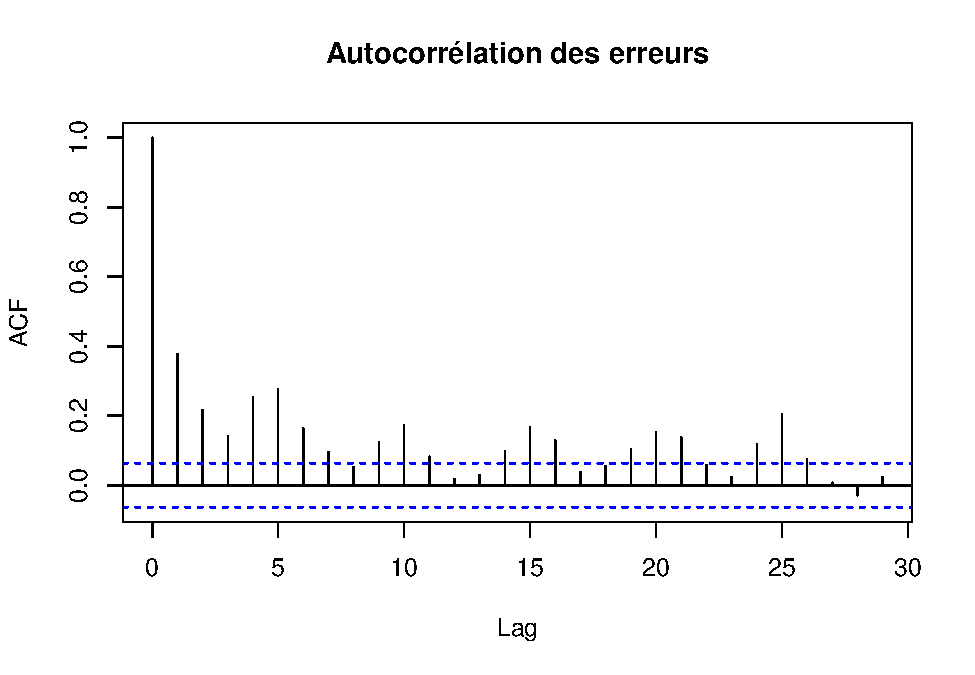
\includegraphics{rmd_final_files/figure-latex/unnamed-chunk-14-1.pdf}

On remarque que plusieurs barres sortent de l'intervalle de confiance,
ce qui vient soutenir la conclusion\\
du test de Durbin-Watson selon laquelle les erreurs sont
\textbf{autocorrélées}.

\textbf{Test de Breusch-Pagan}

\begin{longtable}[]{@{}ll@{}}
\caption{Breusch-Pagan Test Results}\tabularnewline
\toprule\noalign{}
Description & Valeur \\
\midrule\noalign{}
\endfirsthead
\toprule\noalign{}
Description & Valeur \\
\midrule\noalign{}
\endhead
\bottomrule\noalign{}
\endlastfoot
Breusch-Pagan statistic (BP) & 140.25 \\
Degrés de liberté (df) & 8 \\
p-value & \textless{} 2.2e-16 \\
\end{longtable}

\begin{itemize}
\tightlist
\item
  \textbf{Breusch-Pagan statistic (BP)} : \textbf{140.25}\\
\item
  \textbf{Degrés de liberté (df)} : \textbf{8}\\
\item
  \textbf{p-value} : \textbf{\textless{} 2.2e-16}
\end{itemize}

D'après les résultats du \textbf{test de Breusch-Pagan}, nous acceptons
l'\textbf{hypothèse H1},\\
ce qui signifie que \textbf{l'erreur est hétéroscédastique}. Cela
indique qu'il existe une \textbf{dépendance}\\
entre la variance des erreurs et les \textbf{variables explicatives}.

\textbf{Test de Normalité de Shapiro-Wilk}

\begin{longtable}[]{@{}ll@{}}
\caption{Shapiro-Wilk Normality Test Results}\tabularnewline
\toprule\noalign{}
Description & Valeur \\
\midrule\noalign{}
\endfirsthead
\toprule\noalign{}
Description & Valeur \\
\midrule\noalign{}
\endhead
\bottomrule\noalign{}
\endlastfoot
Shapiro-Wilk statistic (W) & 0.99532 \\
p-value & 0.002986 \\
\end{longtable}

\begin{itemize}
\tightlist
\item
  \textbf{Shapiro-Wilk statistic (W)} : \textbf{0.99532}\\
\item
  \textbf{p-value} : \textbf{0.002986}
\end{itemize}

D'après les résultats du \textbf{test de Shapiro-Wilk}, la p-value est
\textbf{inférieure au seuil de 5 \%}.\\
Nous rejetons donc l'\textbf{hypothèse nulle (H0)} de normalité des
erreurs.\\
Par conséquent, \textbf{les erreurs ne suivent pas une distribution
normale}.

\begin{longtable}[]{@{}rrrrrr@{}}
\caption{A tibble: 6 x 6}\tabularnewline
\toprule\noalign{}
.fitted & .resid & .hat & .sigma & .cooksd & .std.resid \\
\midrule\noalign{}
\endfirsthead
\toprule\noalign{}
.fitted & .resid & .hat & .sigma & .cooksd & .std.resid \\
\midrule\noalign{}
\endhead
\bottomrule\noalign{}
\endlastfoot
53.5 & 26.50 & 0.01370 & 10.4 & 0.010200 & 2.570 \\
53.7 & 8.14 & 0.01290 & 10.4 & 0.000902 & 0.788 \\
56.8 & -16.50 & 0.01700 & 10.4 & 0.004950 & -1.600 \\
67.7 & -26.60 & 0.02870 & 10.4 & 0.022100 & -2.600 \\
60.9 & -16.60 & 0.03060 & 10.4 & 0.009230 & -1.620 \\
26.9 & 20.20 & 0.00694 & 10.4 & 0.002940 & 1.950 \\
\end{longtable}

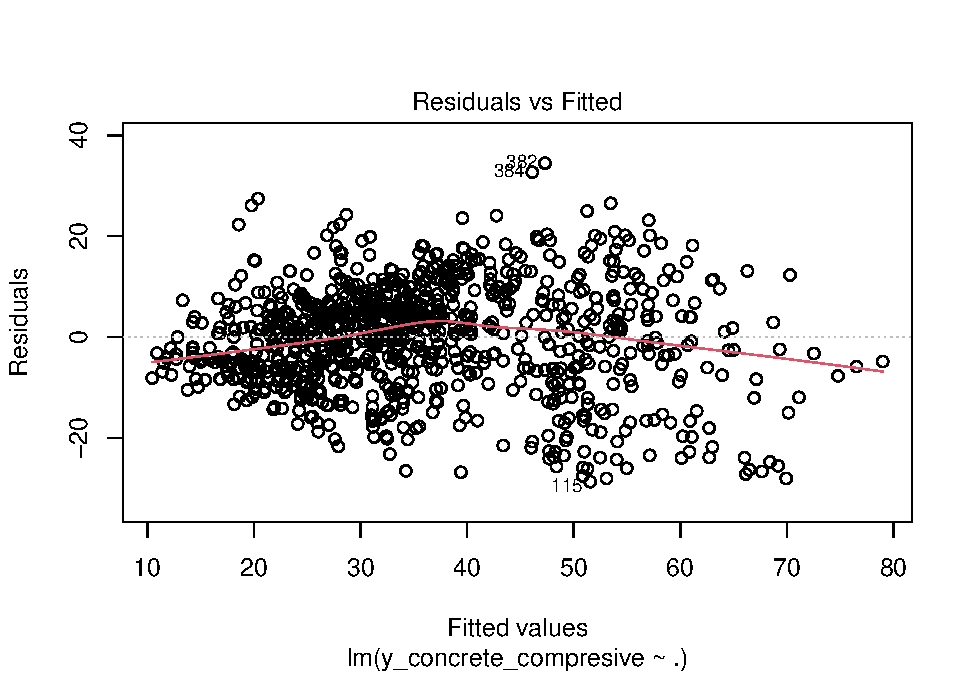
\includegraphics{rmd_final_files/figure-latex/unnamed-chunk-18-1.pdf}

D'après ce plot, il \textbf{n'existe aucune linéarité} entre la variable
réponse et les variables explicatives.\\
La \textbf{courbe rouge n'est pas horizontale}, ce qui indique que la
relation \textbf{n'est pas linéaire}.

Les observations \textbf{382, 384 et 115} sont les \textbf{bétons
présentant les plus grandes valeurs en termes de résidus}.

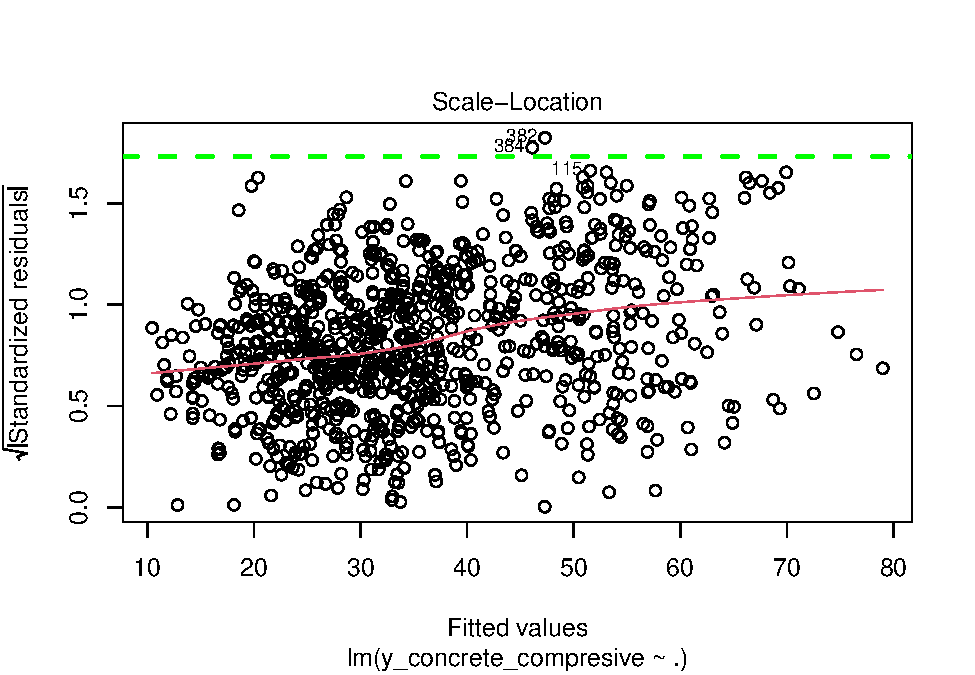
\includegraphics{rmd_final_files/figure-latex/unnamed-chunk-19-1.pdf}

Dans notre cas, la \textbf{courbe rouge n'est pas horizontale} et ne
sépare pas les points de manière homogène\\
de part et d'autre. Cela indique que \textbf{les erreurs ne sont pas
homogènes}, ce qui confirme la conclusion\\
du \textbf{test de Breusch-Pagan}.

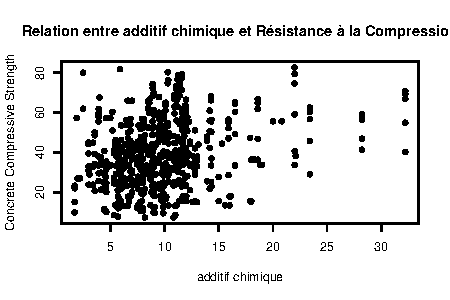
\includegraphics{rmd_final_files/figure-latex/unnamed-chunk-20-1.pdf}

Ce plot de l'\textbf{hypothèse de normalité} montre que plusieurs points
\textbf{ne suivent pas la ligne},\\
bien qu'ils en soient proches.

Cela confirme les résultats du \textbf{test de normalité de
Shapiro-Wilk},\\
indiquant que les erreurs \textbf{ne suivent pas une distribution
normale}.

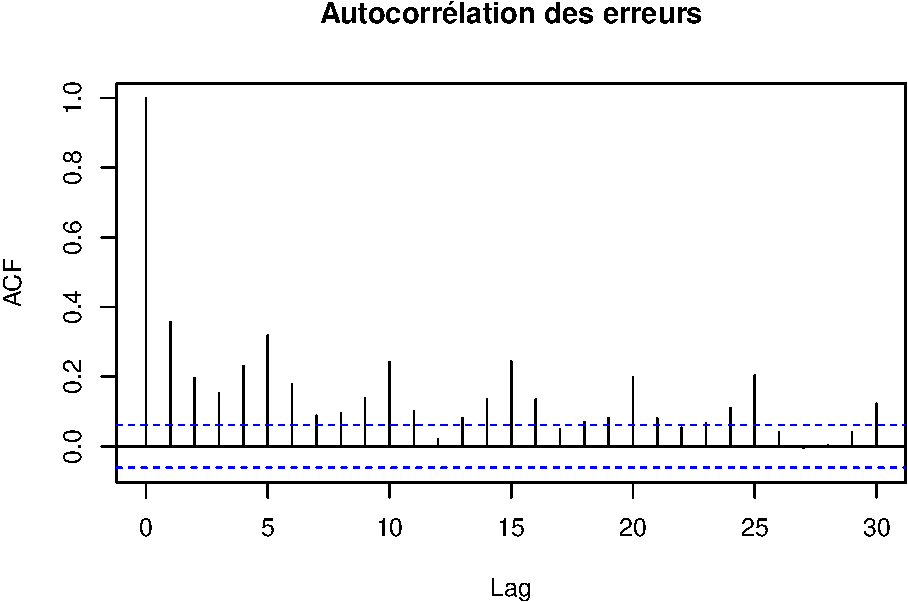
\includegraphics{rmd_final_files/figure-latex/unnamed-chunk-21-1.pdf}

Tous les points situés \textbf{à droite de la droite verticale bleue}
sont des \textbf{points leviers extrêmes},\\
c'est-à-dire des \textbf{valeurs extrêmes des variables explicatives}.

De plus, tous les points \textbf{en dehors de l'intervalle formé par les
pointillés jaunes} sont des \textbf{outliers},\\
c'est-à-dire des \textbf{valeurs extrêmes de la variable cible}.

Dans notre cas, nous avons \textbf{deux outliers} et \textbf{plusieurs
points leviers extrêmes}.

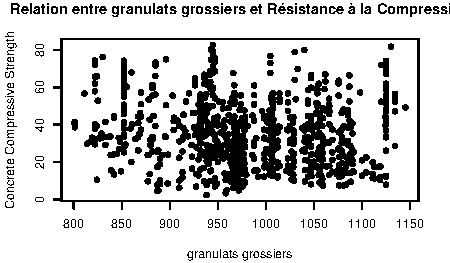
\includegraphics{rmd_final_files/figure-latex/unnamed-chunk-22-1.pdf}

Suite à l'observation des résultats donnés par le graphique, on remarque
que \textbf{plusieurs points dépassent la ligne}\\
formée par les \textbf{pointillés rouges}, qui représente le seuil à
partir duquel un point est \textbf{considéré comme influent}.

Les \textbf{bétons 57, 225 et 611} sont les \textbf{plus influents}.

\section{Conclusion}\label{conclusion}

\section{Annexe}\label{annexe}

\subsection{Analyse univariée}\label{analyse-univariuxe9e}

\subsubsection{\texorpdfstring{Fig 1 : Histogramme pour la variable
\texttt{Cement}}{Fig 1 : Histogramme pour la variable Cement}}\label{fig-1-histogramme-pour-la-variable-cement}

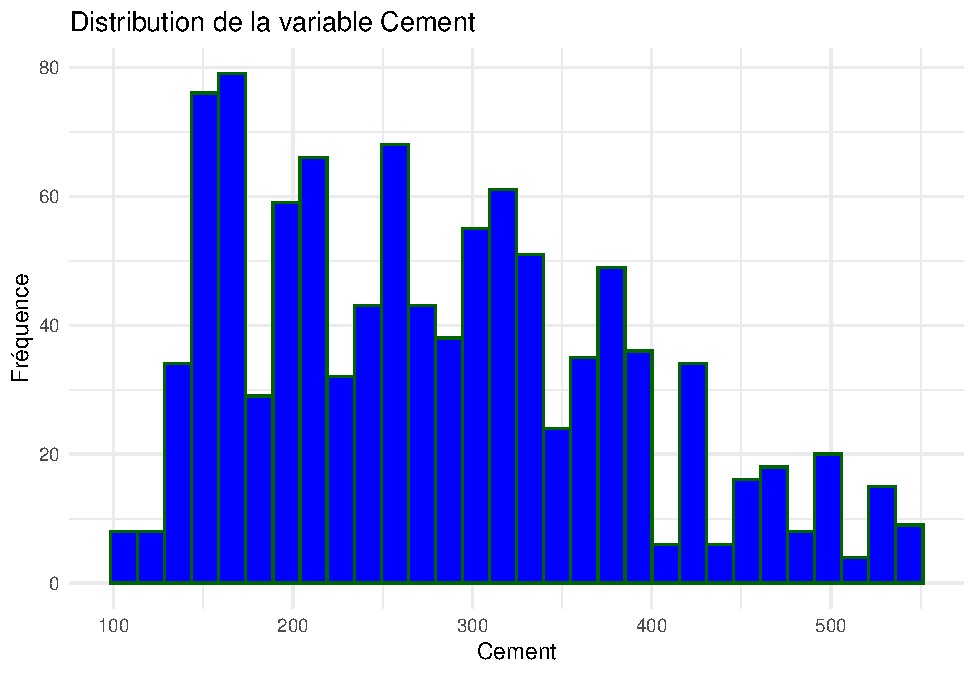
\includegraphics{rmd_final_files/figure-latex/unnamed-chunk-23-1.pdf}

\subsubsection{\texorpdfstring{Fig 2 : Histogramme pour la variable
\texttt{Blast\ Furnace\ Slag}}{Fig 2 : Histogramme pour la variable Blast Furnace Slag}}\label{fig-2-histogramme-pour-la-variable-blast-furnace-slag}

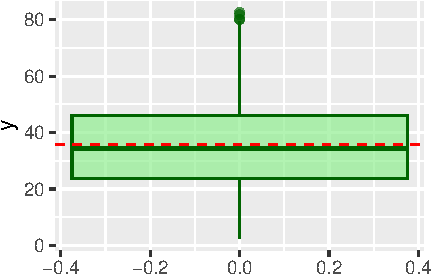
\includegraphics{rmd_final_files/figure-latex/unnamed-chunk-24-1.pdf}

\subsubsection{\texorpdfstring{Fig 3 :Histogramme pour la variable
\texttt{Fly\ Ash}}{Fig 3 :Histogramme pour la variable Fly Ash}}\label{fig-3-histogramme-pour-la-variable-fly-ash}

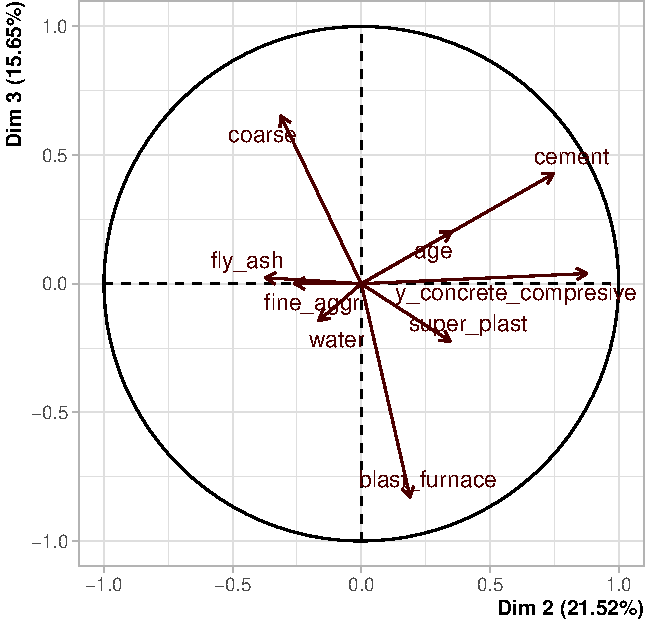
\includegraphics{rmd_final_files/figure-latex/unnamed-chunk-25-1.pdf}

\subsubsection{\texorpdfstring{Fig 4: Histogramme pour la variable
\texttt{Water}}{Fig 4: Histogramme pour la variable Water}}\label{fig-4-histogramme-pour-la-variable-water}

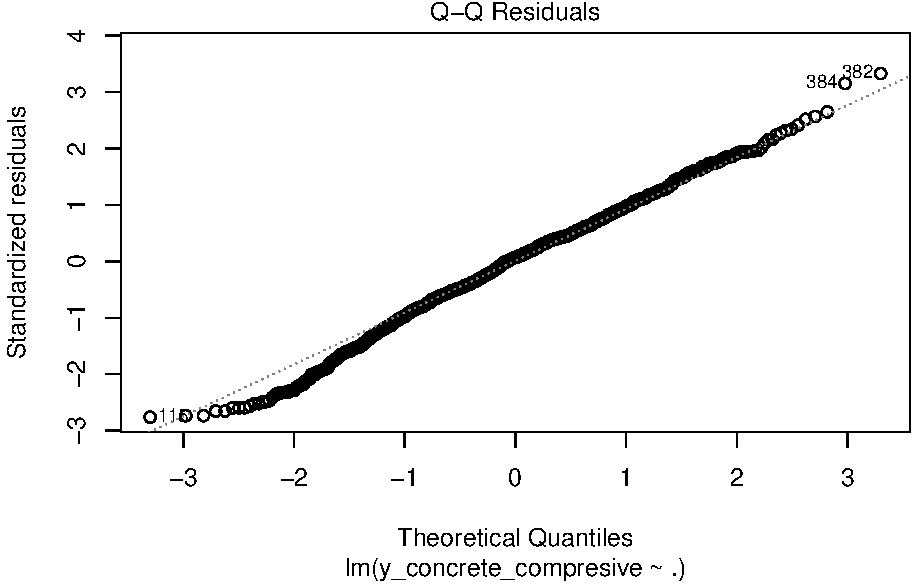
\includegraphics{rmd_final_files/figure-latex/unnamed-chunk-26-1.pdf}

\subsubsection{\texorpdfstring{Fig 5 : Histogramme pour la variable
\texttt{Superplasticizer}}{Fig 5 : Histogramme pour la variable Superplasticizer}}\label{fig-5-histogramme-pour-la-variable-superplasticizer}

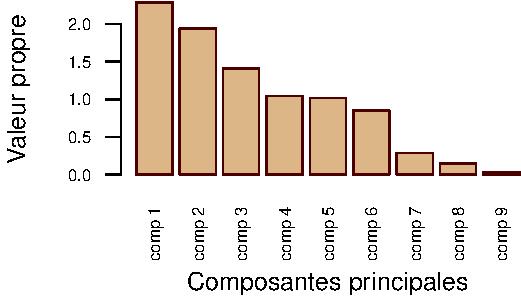
\includegraphics{rmd_final_files/figure-latex/unnamed-chunk-27-1.pdf}

\subsubsection{\texorpdfstring{Fig 6 : Histogramme pour la variable
\texttt{Coarse\ Aggregate}}{Fig 6 : Histogramme pour la variable Coarse Aggregate}}\label{fig-6-histogramme-pour-la-variable-coarse-aggregate}

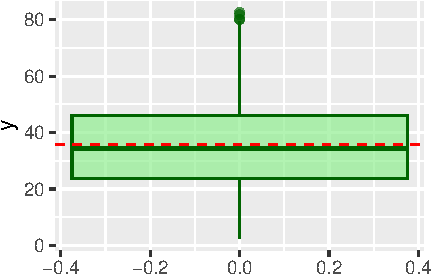
\includegraphics{rmd_final_files/figure-latex/unnamed-chunk-28-1.pdf}

\subsubsection{\texorpdfstring{Fig 7 : Histogramme pour la variable
\texttt{Fine\ Aggregate}}{Fig 7 : Histogramme pour la variable Fine Aggregate}}\label{fig-7-histogramme-pour-la-variable-fine-aggregate}

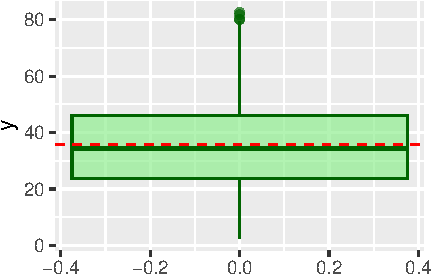
\includegraphics{rmd_final_files/figure-latex/unnamed-chunk-29-1.pdf}

\subsubsection{\texorpdfstring{Fig 8 : Histogramme pour la variable
\texttt{Age}}{Fig 8 : Histogramme pour la variable Age}}\label{fig-8-histogramme-pour-la-variable-age}

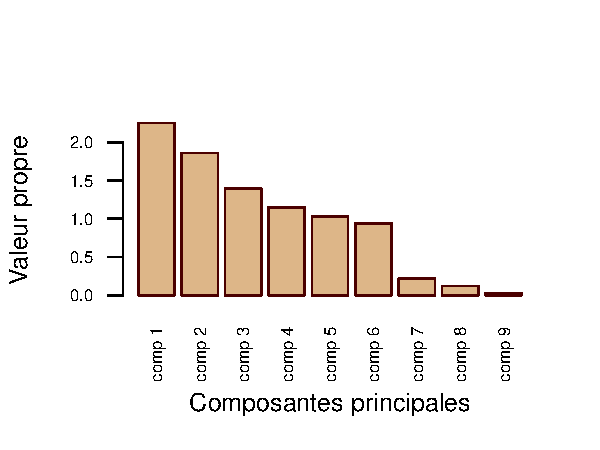
\includegraphics{rmd_final_files/figure-latex/unnamed-chunk-30-1.pdf}

\subsubsection{\texorpdfstring{Fig 9 : Histogramme pour la variable
\texttt{Concrete\ Compressive\ Strength}}{Fig 9 : Histogramme pour la variable Concrete Compressive Strength}}\label{fig-9-histogramme-pour-la-variable-concrete-compressive-strength}

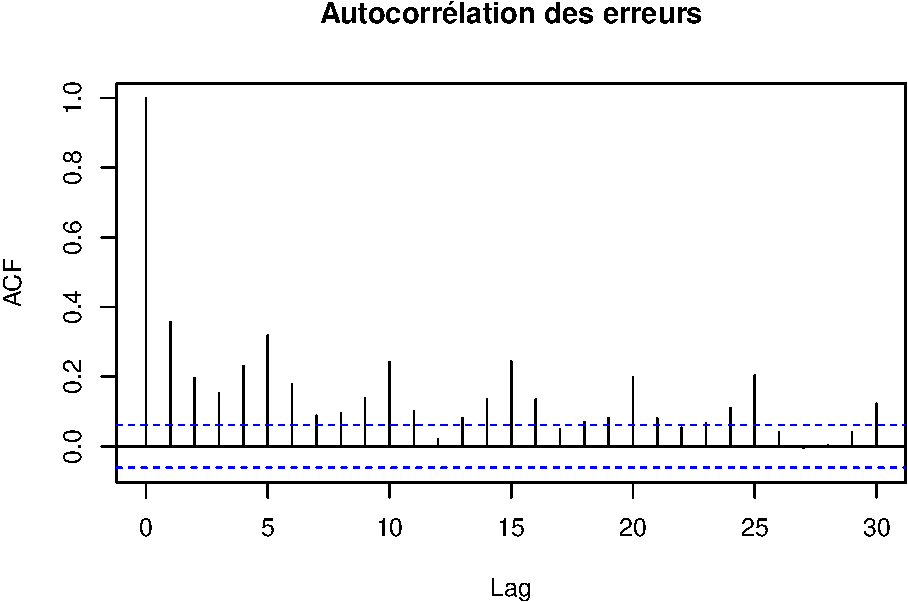
\includegraphics{rmd_final_files/figure-latex/unnamed-chunk-31-1.pdf}

\subsubsection{Fig 10 : Détection des valeurs aberrantes
(Boxplots)}\label{fig-10-duxe9tection-des-valeurs-aberrantes-boxplots}

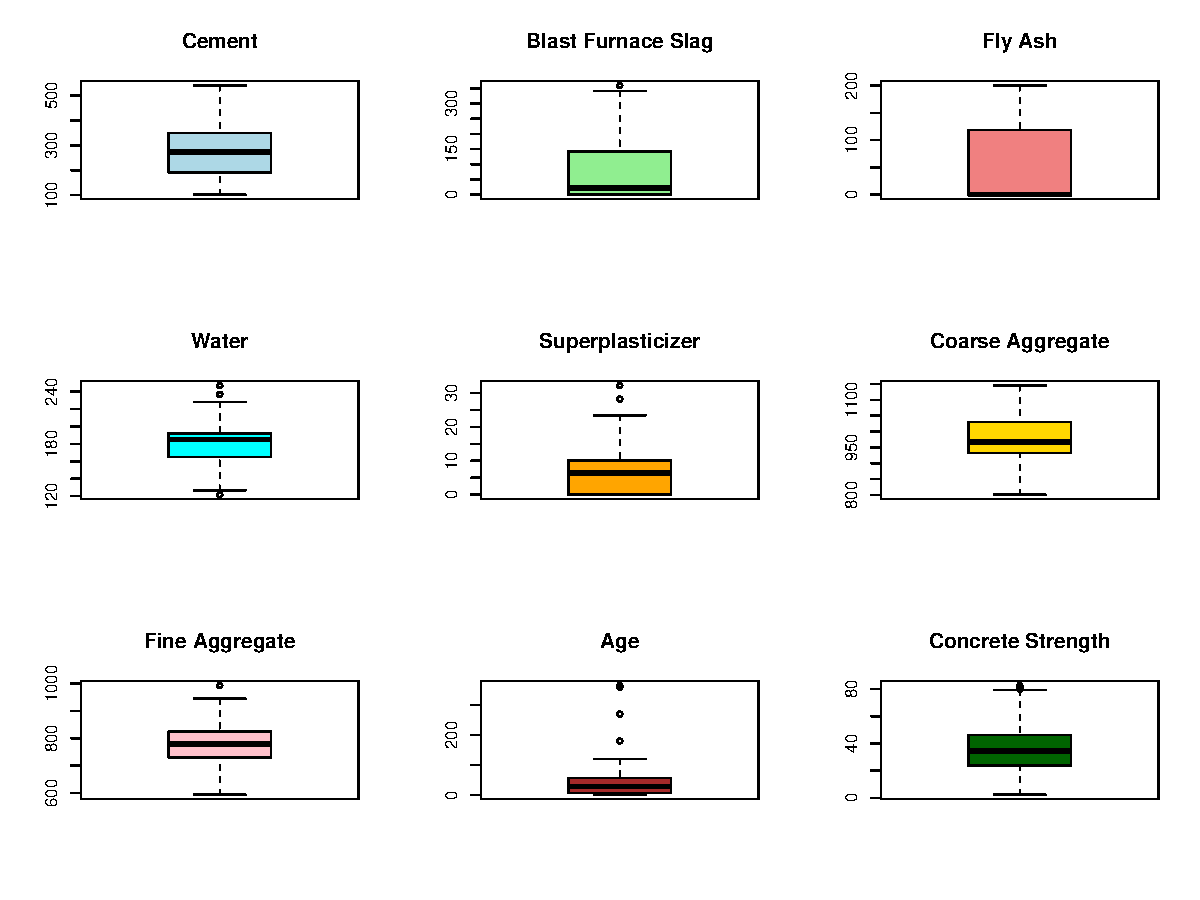
\includegraphics{rmd_final_files/figure-latex/boxplots_outliers-1.pdf}

\subsection{Analyse bivariee}\label{analyse-bivariee}

\subsubsection{Fig 11 :Matrice de
correlation}\label{fig-11-matrice-de-correlation}

\begin{verbatim}
##                            cement blast_furnace      fly_ash       water
## cement                 1.00000000   -0.27519344 -0.397475440 -0.08154361
## blast_furnace         -0.27519344    1.00000000 -0.323569468  0.10728594
## fly_ash               -0.39747544   -0.32356947  1.000000000 -0.25704400
## water                 -0.08154361    0.10728594 -0.257043997  1.00000000
## super_plast            0.09277137    0.04337574  0.377339559 -0.65746444
## coarse                -0.10935604   -0.28399823 -0.009976788 -0.18231167
## fine_aggr             -0.22272017   -0.28159326  0.079076351 -0.45063498
## age                    0.08194726   -0.04424580 -0.154370165  0.27760443
## y_concrete_compresive  0.49783272    0.13482445 -0.105753348 -0.28961348
##                       super_plast       coarse   fine_aggr          age
## cement                 0.09277137 -0.109356039 -0.22272017  0.081947264
## blast_furnace          0.04337574 -0.283998230 -0.28159326 -0.044245801
## fly_ash                0.37733956 -0.009976788  0.07907635 -0.154370165
## water                 -0.65746444 -0.182311668 -0.45063498  0.277604429
## super_plast            1.00000000 -0.266302755  0.22250149 -0.192716518
## coarse                -0.26630276  1.000000000 -0.17850575 -0.003015507
## fine_aggr              0.22250149 -0.178505755  1.00000000 -0.156094049
## age                   -0.19271652 -0.003015507 -0.15609405  1.000000000
## y_concrete_compresive  0.36610230 -0.164927821 -0.16724896  0.328876976
##                       y_concrete_compresive
## cement                            0.4978327
## blast_furnace                     0.1348244
## fly_ash                          -0.1057533
## water                            -0.2896135
## super_plast                       0.3661023
## coarse                           -0.1649278
## fine_aggr                        -0.1672490
## age                               0.3288770
## y_concrete_compresive             1.0000000
\end{verbatim}

\begin{center}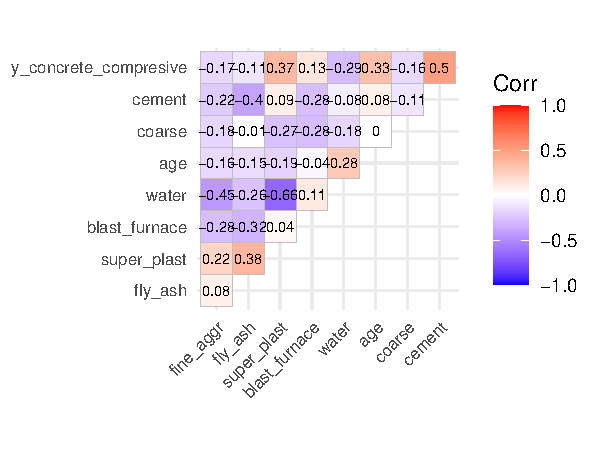
\includegraphics{rmd_final_files/figure-latex/corr_y-1} \end{center}

\subsubsection{Fig 12 : Nuage des points entre le ciment et la
resistance à la
compression}\label{fig-12-nuage-des-points-entre-le-ciment-et-la-resistance-uxe0-la-compression}

\begin{center}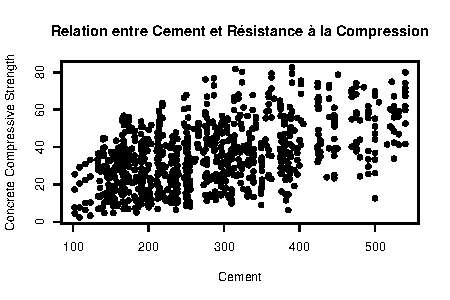
\includegraphics{rmd_final_files/figure-latex/unnamed-chunk-32-1} \end{center}

\subsubsection{Fig 13 : Relation entre l'eau et Super
plasticizer}\label{fig-13-relation-entre-leau-et-super-plasticizer}

\begin{center}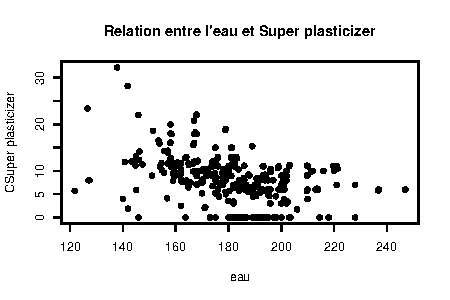
\includegraphics{rmd_final_files/figure-latex/unnamed-chunk-33-1} \end{center}

\subsubsection{Fig 14 : Relation entre l'age et la
resistance}\label{fig-14-relation-entre-lage-et-la-resistance}

\begin{center}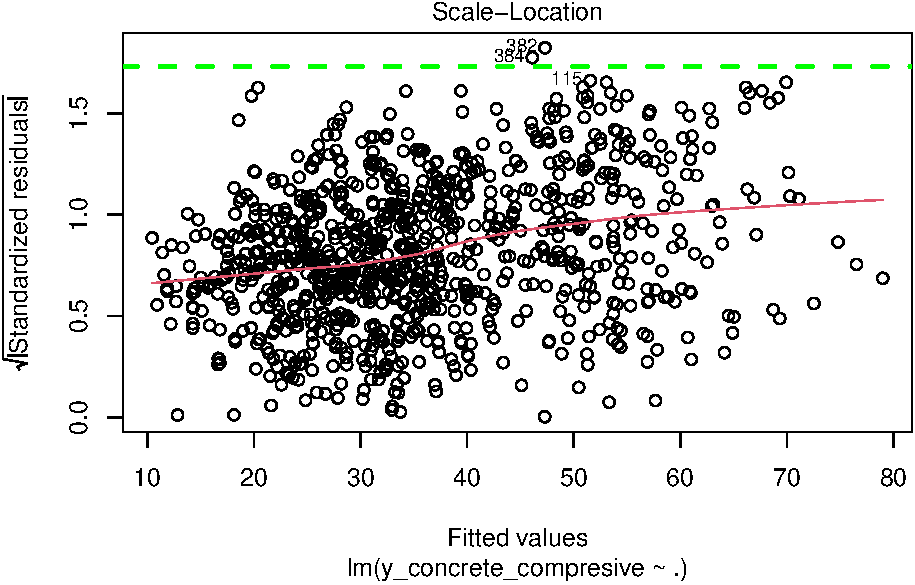
\includegraphics{rmd_final_files/figure-latex/unnamed-chunk-34-1} \end{center}

\subsubsection{Fig 15 : Relation entre laitier haut fourneau et
Résistance à la
Compression}\label{fig-15-relation-entre-laitier-haut-fourneau-et-ruxe9sistance-uxe0-la-compression}

\begin{center}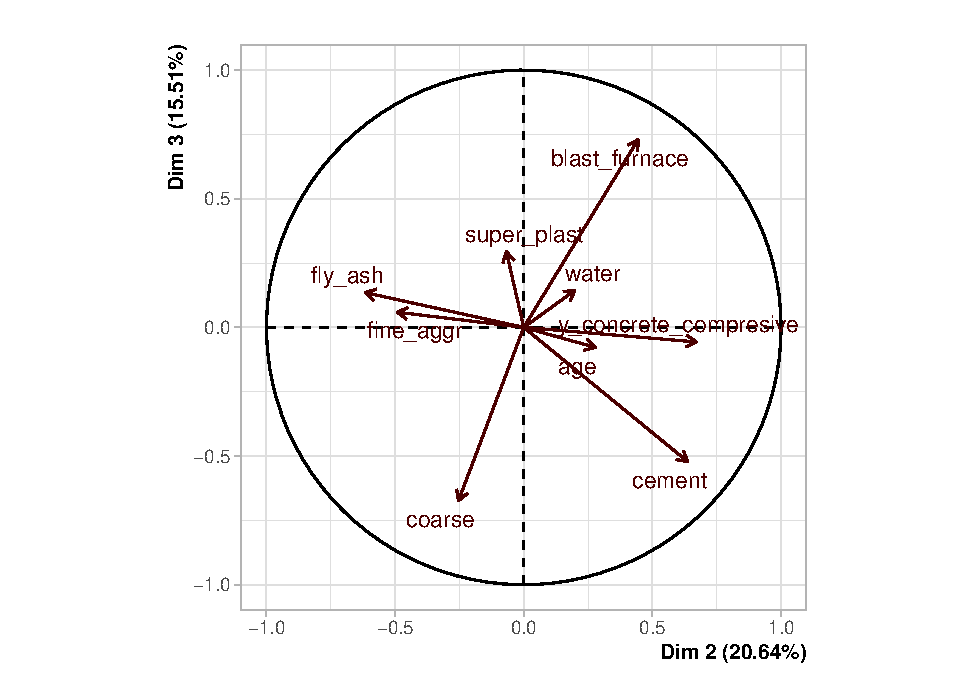
\includegraphics{rmd_final_files/figure-latex/unnamed-chunk-35-1} \end{center}

\subsubsection{Fig 16 : Relation entre Cendres volantes et Résistance à
la
Compression}\label{fig-16-relation-entre-cendres-volantes-et-ruxe9sistance-uxe0-la-compression}

\begin{center}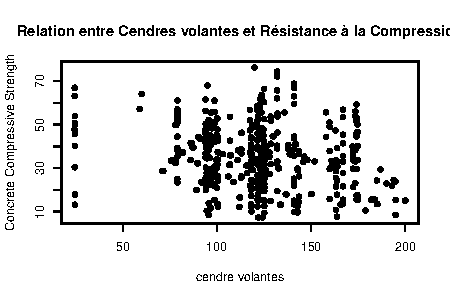
\includegraphics{rmd_final_files/figure-latex/unnamed-chunk-36-1} \end{center}

\subsubsection{Fig 17 : Relation entre eau et Résistance à la
Compression}\label{fig-17-relation-entre-eau-et-ruxe9sistance-uxe0-la-compression}

\begin{center}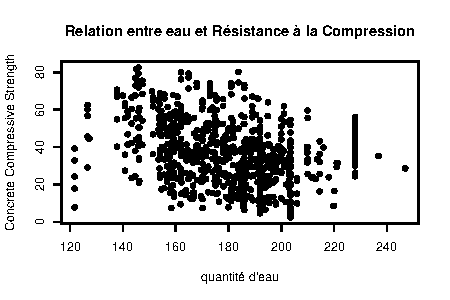
\includegraphics{rmd_final_files/figure-latex/unnamed-chunk-37-1} \end{center}

\subsubsection{Fig 18 : Relation entre additif chimique et Résistance à
la
Compression}\label{fig-18-relation-entre-additif-chimique-et-ruxe9sistance-uxe0-la-compression}

\begin{center}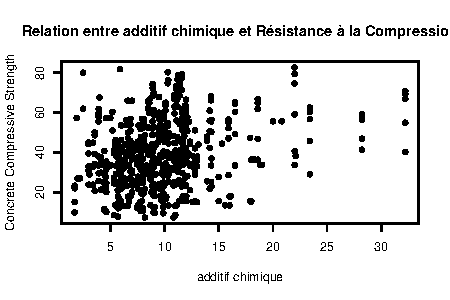
\includegraphics{rmd_final_files/figure-latex/unnamed-chunk-38-1} \end{center}

\subsubsection{Fig 19 : Relation entre granulats grossiers et Résistance
à la
Compression}\label{fig-19-relation-entre-granulats-grossiers-et-ruxe9sistance-uxe0-la-compression}

\begin{center}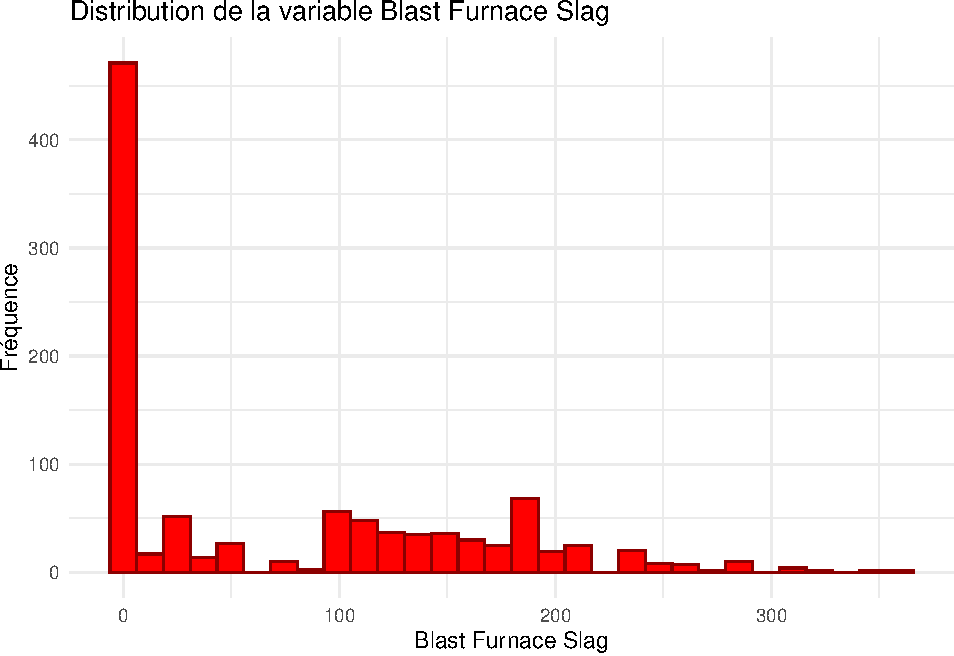
\includegraphics{rmd_final_files/figure-latex/unnamed-chunk-39-1} \end{center}

\subsubsection{Fig 20 : Relation entre granulats fins et la resistance à
la
compression}\label{fig-20-relation-entre-granulats-fins-et-la-resistance-uxe0-la-compression}

\begin{center}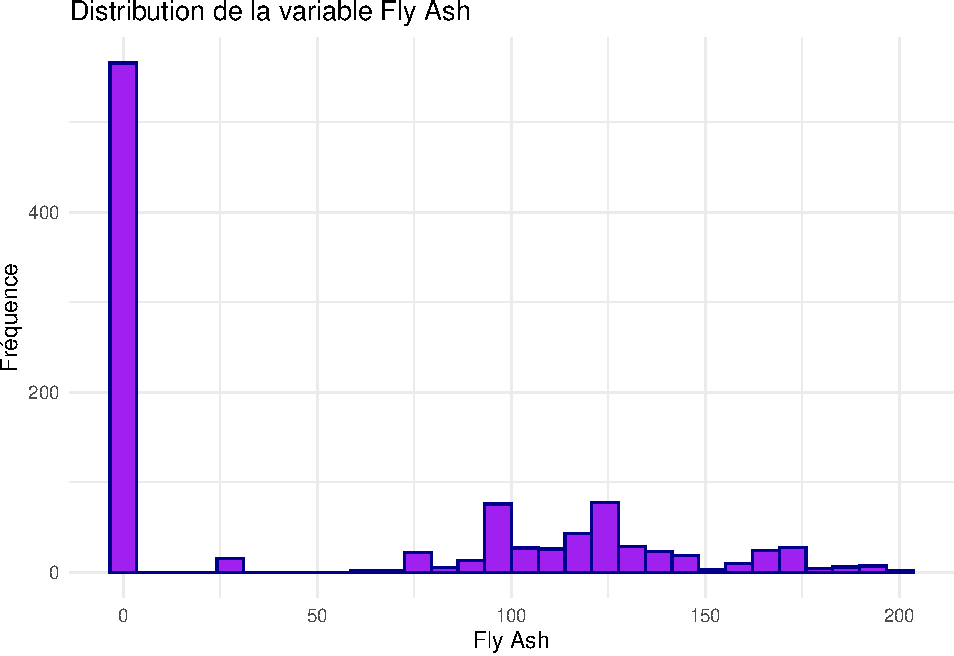
\includegraphics{rmd_final_files/figure-latex/unnamed-chunk-40-1} \end{center}

test corrrelation entre variable à expliquer et \texttt{cement}

\begin{Shaded}
\begin{Highlighting}[]
\FunctionTok{cor.test}\NormalTok{(bdd}\SpecialCharTok{$}\NormalTok{cement, bdd}\SpecialCharTok{$}\NormalTok{y\_concrete\_compresive, }\AttributeTok{method =} \StringTok{"pearson"}\NormalTok{)}
\end{Highlighting}
\end{Shaded}

\begin{verbatim}
## 
##  Pearson's product-moment correlation
## 
## data:  bdd$cement and bdd$y_concrete_compresive
## t = 18.405, df = 1028, p-value < 2.2e-16
## alternative hypothesis: true correlation is not equal to 0
## 95 percent confidence interval:
##  0.4504473 0.5424213
## sample estimates:
##       cor 
## 0.4978327
\end{verbatim}

\begin{Shaded}
\begin{Highlighting}[]
\CommentTok{\#test de pearson car ont une distribution pseudo{-}normale}
\end{Highlighting}
\end{Shaded}

test de correlation entre variable \texttt{water} et
\texttt{SuperPlasticizer}

\begin{Shaded}
\begin{Highlighting}[]
\FunctionTok{cor.test}\NormalTok{(bdd}\SpecialCharTok{$}\NormalTok{water, bdd}\SpecialCharTok{$}\NormalTok{super\_plast, }\AttributeTok{method =} \StringTok{"kendall"}\NormalTok{)}
\end{Highlighting}
\end{Shaded}

\begin{verbatim}
## 
##  Kendall's rank correlation tau
## 
## data:  bdd$water and bdd$super_plast
## z = -23.914, p-value < 2.2e-16
## alternative hypothesis: true tau is not equal to 0
## sample estimates:
##       tau 
## -0.528651
\end{verbatim}

\begin{Shaded}
\begin{Highlighting}[]
\CommentTok{\#test de Kendall car n\textquotesingle{}ont pas de distribution pseudo{-} normale}
\end{Highlighting}
\end{Shaded}

test de correlation entre variable \texttt{water} et \texttt{y}

\begin{Shaded}
\begin{Highlighting}[]
\FunctionTok{cor.test}\NormalTok{(bdd}\SpecialCharTok{$}\NormalTok{age, bdd}\SpecialCharTok{$}\NormalTok{y\_concrete\_compresive, }\AttributeTok{method =} \StringTok{"kendall"}\NormalTok{)}
\end{Highlighting}
\end{Shaded}

\begin{verbatim}
## 
##  Kendall's rank correlation tau
## 
## data:  bdd$age and bdd$y_concrete_compresive
## z = 19.826, p-value < 2.2e-16
## alternative hypothesis: true tau is not equal to 0
## sample estimates:
##       tau 
## 0.4490164
\end{verbatim}

\begin{Shaded}
\begin{Highlighting}[]
\CommentTok{\#test de Kendall car n\textquotesingle{}ont pas de distribution pseudo{-} normale}
\end{Highlighting}
\end{Shaded}

\subsection{Analyse multivariée}\label{analyse-multivariuxe9e-1}

\subsubsection{Contribution des
variables}\label{contribution-des-variables}

\begin{Shaded}
\begin{Highlighting}[]
\CommentTok{\# Tableau des contributions des variables}
\FunctionTok{par}\NormalTok{(}\AttributeTok{cex =} \FloatTok{0.65}\NormalTok{)}
\NormalTok{contrib\_var }\OtherTok{\textless{}{-}} \FunctionTok{as.data.frame}\NormalTok{(res\_pca}\SpecialCharTok{$}\NormalTok{var}\SpecialCharTok{$}\NormalTok{contrib)}
\FunctionTok{print}\NormalTok{(contrib\_var)}
\end{Highlighting}
\end{Shaded}

\begin{verbatim}
##                            Dim.1      Dim.2      Dim.3      Dim.4      Dim.5
## cement                 1.8570924 21.8162521 19.4630539 17.0024498  0.3034758
## blast_furnace          1.3854568 10.6144114 38.1264598  0.8844007  4.7645646
## fly_ash                7.2754889 20.3973975  1.3084478  9.8815857  4.0570219
## water                 28.2000179  2.1202816  1.4847945  2.0723167  4.4435413
## super_plast           30.7756668  0.2472336  6.2022982  0.9015953  8.4701606
## coarse                 0.8939835  3.4632950 32.5054492 12.5162699 10.6005496
## fine_aggr              4.8648268 13.0123250  0.2499000 13.1394718 39.0454823
## age                    5.5749786  4.1403732  0.4309223 40.7207759 28.1887145
## y_concrete_compresive 19.1724883 24.1884306  0.2286743  2.8811343  0.1264894
\end{verbatim}

\subsubsection{\texorpdfstring{Tableau des \(cos^2\) des variables
sur}{Tableau des cos\^{}2 des variables sur}}\label{tableau-des-cos2-des-variables-sur}

\begin{Shaded}
\begin{Highlighting}[]
\CommentTok{\# Tableau des cos² des variables}
\FunctionTok{par}\NormalTok{(}\AttributeTok{cex =} \FloatTok{0.65}\NormalTok{)}
\NormalTok{cos2\_var }\OtherTok{\textless{}{-}} \FunctionTok{as.data.frame}\NormalTok{(res\_pca}\SpecialCharTok{$}\NormalTok{var}\SpecialCharTok{$}\NormalTok{cos2)}
\FunctionTok{print}\NormalTok{(cos2\_var)}
\end{Highlighting}
\end{Shaded}

\begin{verbatim}
##                            Dim.1       Dim.2       Dim.3      Dim.4       Dim.5
## cement                0.04181872 0.405352873 0.271676732 0.19539670 0.003132659
## blast_furnace         0.03119825 0.197219125 0.532191509 0.01016377 0.049182696
## fly_ash               0.16383224 0.378990105 0.018264082 0.11356182 0.041879015
## water                 0.63501880 0.039395503 0.020725633 0.02381562 0.045868900
## super_plast           0.69301824 0.004593679 0.086575320 0.01036137 0.087434082
## coarse                0.02013106 0.064349119 0.453730143 0.14384032 0.109425235
## fine_aggr             0.10954803 0.241773118 0.003488251 0.15100232 0.403050903
## age                   0.12553950 0.076929445 0.006015067 0.46797404 0.290980829
## y_concrete_compresive 0.43173343 0.449428700 0.003191970 0.03311077 0.001305699
\end{verbatim}

\subsubsection{Fig 21 : PCA sur la dimension
1-3}\label{fig-21-pca-sur-la-dimension-1-3}

\begin{Shaded}
\begin{Highlighting}[]
\FunctionTok{plot.PCA}\NormalTok{(}
\NormalTok{    res\_pca,}
    \AttributeTok{axes =} \FunctionTok{c}\NormalTok{(}\DecValTok{1}\NormalTok{, }\DecValTok{3}\NormalTok{),             }\CommentTok{\# On se concentre sur les axes 2 et 3}
    \AttributeTok{choix =} \StringTok{"var"}\NormalTok{,              }\CommentTok{\# Afficher les variables dans le plan factoriel}
    \AttributeTok{col.var =} \StringTok{"\#4B0000"}\NormalTok{,        }\CommentTok{\# Couleur des variables alignée au style}
    \AttributeTok{col.quanti.sup =} \StringTok{"\#0000FF"}\NormalTok{, }\CommentTok{\# Couleur pour la variable quantitative supplémentaire}
    \AttributeTok{label =} \StringTok{"all"}\NormalTok{,}
    \AttributeTok{title =} \StringTok{""}\NormalTok{,}
    \AttributeTok{addgrid.col =} \StringTok{"\#DDB688"}     \CommentTok{\# Couleur de la grille}
\NormalTok{  )}
\end{Highlighting}
\end{Shaded}

\begin{center}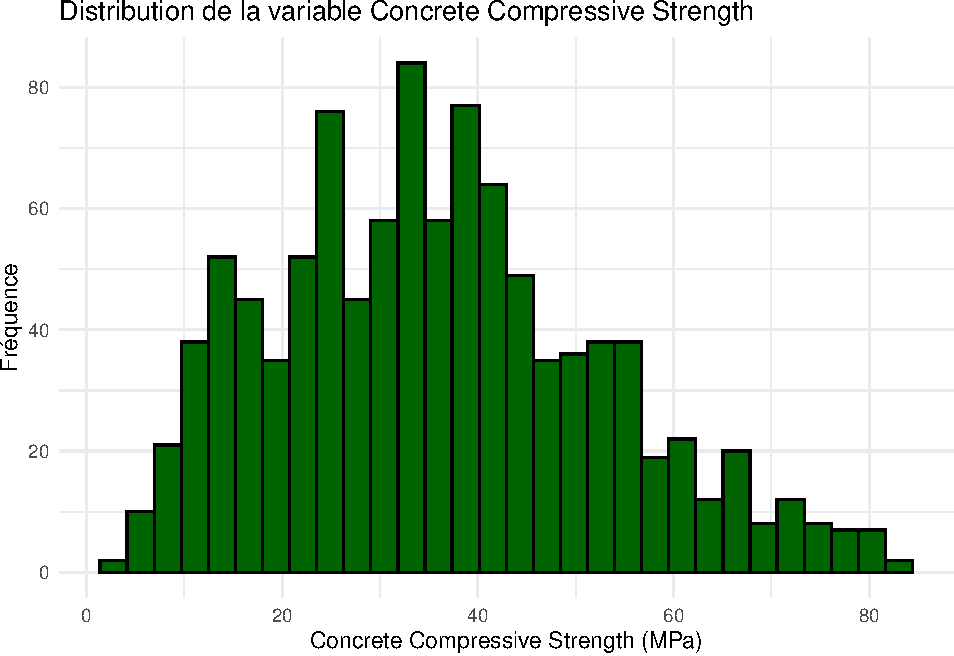
\includegraphics{rmd_final_files/figure-latex/unnamed-chunk-46-1} \end{center}

\subsubsection{Fig 22 : PCA sur la dimension
2-3}\label{fig-22-pca-sur-la-dimension-2-3}

\begin{Shaded}
\begin{Highlighting}[]
\CommentTok{\# Représentation des variables sur le plan factoriel (axes 1 et 3)}
\FunctionTok{plot.PCA}\NormalTok{(}
\NormalTok{  res\_pca,}
  \AttributeTok{axes =} \FunctionTok{c}\NormalTok{(}\DecValTok{2}\NormalTok{, }\DecValTok{3}\NormalTok{),             }\CommentTok{\# On se concentre sur les 2 premiers axes}
  \AttributeTok{choix =} \StringTok{"var"}\NormalTok{,              }\CommentTok{\# Afficher les variables dans le plan factoriel}
  \AttributeTok{col.var =} \StringTok{"\#4B0000"}\NormalTok{,        }\CommentTok{\# Couleur des variables alignée au style}
  \AttributeTok{col.quanti.sup =} \StringTok{"\#0000FF"}\NormalTok{, }\CommentTok{\# Couleur pour la variable quantitative supplémentaire}
  \AttributeTok{label =} \StringTok{"all"}\NormalTok{,}
  \AttributeTok{title =} \StringTok{""}\NormalTok{,}
  \AttributeTok{addgrid.col =} \StringTok{"\#DDB688"}     \CommentTok{\# Couleur de la grille}
\NormalTok{)}
\end{Highlighting}
\end{Shaded}

\begin{center}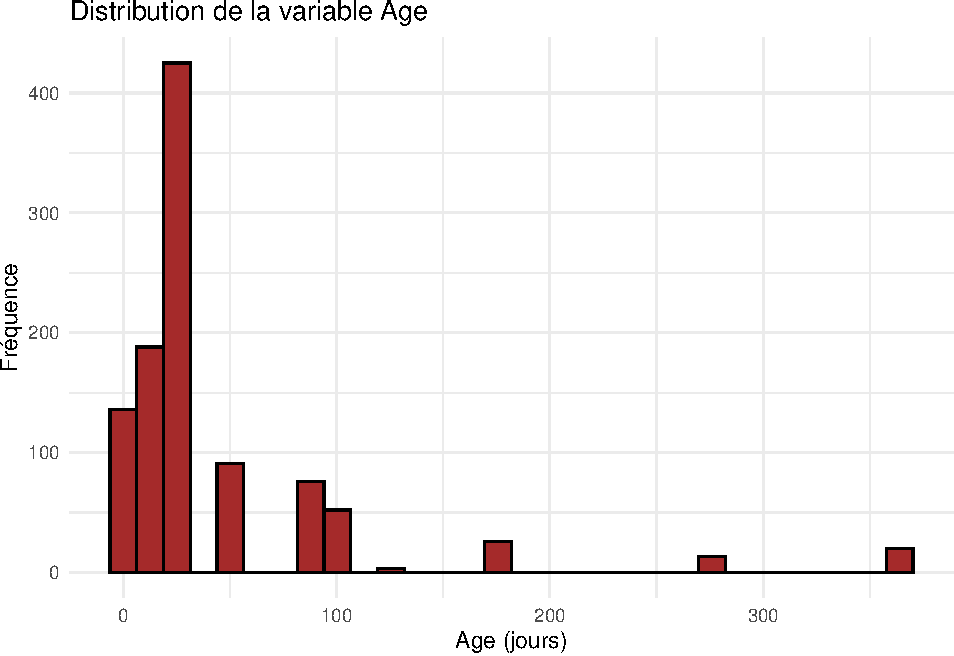
\includegraphics{rmd_final_files/figure-latex/unnamed-chunk-47-1} \end{center}

\end{document}
